% GENERATED FILE. Regenerate it instead of editing diff markup by hand.
% Old source: submission/main-v4-submitted.tex (d68c37599eded0bcbfd280897c84c919cd36565d65030a65ad5233abe02b1d94)
% New source: submission/Final/main-v5-final-draft.tex (f9e453c1043bedb7a41fa3c78867c44fbd593adaf2b378e5cddd14ffbc1ebfc5)
% Command: python3 submission/generate-word-diff.py --old submission/main-v4-submitted.tex --new submission/Final/main-v5-final-draft.tex --output submission/Final/main-v4-submitted-to-v5-final-diff.tex
% !TeX program = xelatex
%%%%%%%%%%%%%%%%%%%%%%%%%%%%%%%%%%%%%%%%%%%%%%%%%
% ACOSUS Paper: An AI-driven Transfer Student Advising System
% Document Class: Article with ACM-style formatting
%%%%%%%%%%%%%%%%%%%%%%%%%%%%%%%%%%%%%%%%%%%%%%%%%

\documentclass[letterpaper,11pt]{article}
\usepackage[margin=1in]{geometry}
\usepackage{xurl}
\usepackage{graphicx}
\usepackage{alltt}
\usepackage{amsmath}
\usepackage{booktabs}
\usepackage{tabularx}
\usepackage[hidelinks, hypertexnames=false]{hyperref}
\hypersetup{pdftitle={ACOSUS: Design and Feasibility Evaluation of an AI-Driven Advising Platform for Transfer Students},pdfauthor={Deep Mandloi, Lizi Zhu, Xiwei Wang}}
\usepackage{float}
\usepackage[font=normalsize,labelfont=normalfont,labelsep=colon,justification=centering,singlelinecheck=false]{caption}
\usepackage{fancyhdr}
\setlength{\headheight}{14pt}
\pagestyle{fancy}
\fancyhf{}
\fancyhead[L]{Mandloi et al.}
\fancyhead[R]{ACOSUS AI-driven transfer advising platform}
\renewcommand{\headrulewidth}{0.4pt}
\renewcommand{\footrulewidth}{0pt}

% Float placement: let large figures/tables share a page with text instead of
% being banished to their own near-empty float pages.
\renewcommand{\topfraction}{0.9}
\renewcommand{\bottomfraction}{0.9}
\renewcommand{\textfraction}{0.08}
\renewcommand{\floatpagefraction}{0.75}
\setcounter{topnumber}{3}
\setcounter{bottomnumber}{2}
\setcounter{totalnumber}{4}

% TikZ packages for diagrams
\usepackage{tikz}
\usetikzlibrary{shapes.geometric, arrows.meta, positioning, fit, backgrounds, calc}

% Define colors for diagrams
\definecolor{targetsurvey}{HTML}{FFF3E0}
\definecolor{factorsurvey}{HTML}{E3F2FD}
\definecolor{processing}{HTML}{F3E5F5}
\definecolor{outputgreen}{HTML}{E8F5E9}
\definecolor{stage1green}{HTML}{D4EDDA}
\definecolor{stage1border}{HTML}{28A745}
\definecolor{stage2yellow}{HTML}{FFF3CD}
\definecolor{stage2border}{HTML}{FFC107}
\definecolor{stage3blue}{HTML}{CCE5FF}
\definecolor{stage3border}{HTML}{007BFF}
\definecolor{framegray}{HTML}{F8F9FA}
\definecolor{frameborder}{HTML}{6C757D}
\definecolor{modelpink}{HTML}{FCE4EC}
% Colors for fig2 (Three-Stage Pipeline)
\definecolor{stage1}{RGB}{76,175,80}
\definecolor{stage2}{RGB}{255,152,0}
\definecolor{stage3}{RGB}{100,149,237}
\definecolor{inputred}{RGB}{183,28,28}
\definecolor{outputviolet}{RGB}{103,58,183}
\definecolor{pipelineborder}{RGB}{120,60,60}
% Colors for fig3 (Survey Processing)
\definecolor{surveyblue}{RGB}{66,133,244}
\definecolor{surveyboxfill}{RGB}{215,232,252}
\definecolor{processorange}{RGB}{234,67,53}
\definecolor{processboxfill}{RGB}{253,232,226}
\definecolor{processboxborder}{RGB}{230,150,100}
\definecolor{modelgreen}{RGB}{15,100,80}
\definecolor{modelboxfill}{RGB}{200,230,225}
\definecolor{modelboxborder}{RGB}{100,180,170}
% Colors for fig4 (System Architecture)
\definecolor{dblue}{RGB}{60,100,180}

% TikZ styles
\tikzset{
    surveybox/.style={rectangle, rounded corners=3pt, minimum width=2.2cm, minimum height=0.8cm, text centered, draw=black!60, font=\scriptsize, text width=2cm, align=center},
    groupbox/.style={rectangle, rounded corners=5pt, draw=black!40, thick},
    arrow/.style={-{Stealth[length=2mm]}, thick, black!70},
    dashedarrow/.style={-{Stealth[length=2mm]}, thick, black!50, dashed},
    stagebox/.style={rectangle, rounded corners=5pt, minimum width=3cm, minimum height=1.8cm, draw, thick, text width=2.8cm, align=center, font=\scriptsize},
    layerbox/.style={rectangle, rounded corners=3pt, minimum width=2cm, minimum height=0.6cm, text centered, draw=black!60, font=\tiny, text width=1.8cm, align=center},
}
\urlstyle{same}
\usepackage{fontspec}
\setmainfont{Arial}
\usepackage{csquotes}
\usepackage[style=apa, backend=biber, sortcites=true, sorting=nyt]{biblatex}
\DeclareLanguageMapping{english}{english-apa}
\addbibresource{references.bib}

\usepackage[english]{babel}

\usepackage{ragged2e}
\newcolumntype{Y}{>{\RaggedRight\hyphenpenalty=10000\exhyphenpenalty=10000\arraybackslash}X}
\setlength{\RaggedRightParindent}{0pt}
\setlength{\RaggedRightRightskip}{0pt plus 4em}
\RaggedRight
\linespread{1.0}
\setlength{\parindent}{0pt}
\setlength{\parskip}{0pt}

\usepackage{titlesec}
% Level 1: ALL CAPS, bold, left-aligned, no displayed number
\titleformat{\section}{\normalfont\bfseries\MakeUppercase}{}{0pt}{}
% Level 2: bold, sentence case, no displayed number
\titleformat{\subsection}{\normalfont\bfseries}{}{0pt}{}
% Level 3: underlined, sentence case, not bold, no displayed number
\titleformat{\subsubsection}{\normalfont}{}{0pt}{\underline}
\titlespacing*{\section}{0pt}{1.5\baselineskip}{0.5\baselineskip}
\titlespacing*{\subsection}{0pt}{1\baselineskip}{0.5\baselineskip}
\titlespacing*{\subsubsection}{0pt}{0.5\baselineskip}{0.5\baselineskip}

% Word-level comparison support generated by generate-word-diff.py.
\usepackage[normalem]{ulem}
\hypersetup{pdftitle={ACOSUS Submitted v4 to Final v5 Comparison}}
\definecolor{diffdelbg}{RGB}{255,214,214}
\definecolor{diffdeltext}{RGB}{145,20,20}
\definecolor{diffaddbg}{RGB}{215,245,220}
\definecolor{diffaddtext}{RGB}{20,110,45}
\setlength{\emergencystretch}{4em}
\newcommand{\DIFdel}[1]{%
  \begingroup\setlength{\fboxsep}{0.5pt}%
  \colorbox{diffdelbg}{\textcolor{diffdeltext}{\sout{#1}}}%
  \endgroup}
\newcommand{\DIFadd}[1]{%
  \begingroup\setlength{\fboxsep}{0.5pt}%
  \colorbox{diffaddbg}{\textcolor{diffaddtext}{#1}}%
  \endgroup}
\newcommand{\DIFdelcite}[1]{%
  \DIFdel{-}\textcolor{diffdeltext}{#1}}
\newcommand{\DIFaddcite}[1]{%
  \DIFadd{+}\textcolor{diffaddtext}{#1}}
\newcommand{\DIFaddedreference}[1]{%
  \par\noindent\begingroup\color{diffaddtext}%
  \textbf{Added citation: }\fullcite{#1}\par\endgroup}
\newcommand{\DIFremovedreference}[1]{%
  \par\noindent\begingroup\color{diffdeltext}%
  \textbf{Removed citation: }\fullcite{#1}\par\endgroup}
\newcommand{\DIFlegend}{%
  \begin{center}\small
  \textbf{Submitted v4 to final v5 comparison}\\[4pt]
  \DIFdel{Removed text}\quad\DIFadd{Added text}\quad Unchanged text
  \end{center}\medskip}

\begin{document}\begin{center}
\textbf{DECISION SCIENCES INSTITUTE}\\[6pt]
\DIFdel{An} \DIFadd{ACOSUS:} \DIFdel{AI-driven} \DIFadd{Design} \DIFadd{and} \DIFadd{Feasibility} \DIFadd{Evaluation} \DIFadd{of} \DIFadd{an} \DIFadd{AI-Driven} \DIFadd{Advising} \DIFadd{Platform} \DIFadd{for} Transfer \DIFdel{Student} \DIFadd{Students}
\\[12pt]
\DIFdel{System:} \DIFadd{Deep} \DIFdel{Design,} \DIFadd{Mandloi}\\
\DIFdel{Implementation,} \DIFadd{Northeastern} \DIFdel{and} \DIFadd{Illinois} \DIFdel{Evaluation} \DIFadd{University}\\
Email: \href{mailto:d-mandloi@neiu.edu}{d-mandloi@neiu.edu}\\[6pt]
Lizi Zhu\\
Northeastern Illinois University\\
Email: \href{mailto:l-zhu2@neiu.edu}{l-zhu2@neiu.edu}\\[6pt]
Shebuti Rayana\\
SUNY at Old Westbury\\
Email: \href{mailto:rayanas@oldwestbury.edu}{rayanas@oldwestbury.edu}\\[6pt]
Palvi Aggarwal\\
University of Texas El Paso\\
Email: \href{mailto:paggarwal@utep.edu}{paggarwal@utep.edu}\\[6pt]
Sherrene Bogle\\
Cal Poly Humboldt\\
Email: \href{mailto:sherrene.bogle@humboldt.edu}{sherrene.bogle@humboldt.edu}\\[6pt]
Yun Wan\\
University of Houston-Downtown\\
Email: \href{mailto:wany@uhd.edu}{wany@uhd.edu}\\[6pt]
Xiwei Wang\\
Northeastern Illinois University\\
Email: \href{mailto:x-wang9@neiu.edu}{x-wang9@neiu.edu}
\end{center}
\DIFlegend

\bigskip

\begin{center}
\textbf{ABSTRACT}
\end{center}

Transfer students face advising challenges that conventional systems do not address well: records are split across institutions, and predictive models are \DIFdel{typically} trained on students who entered as freshmen. We present ACOSUS, an AI-driven advising \DIFdel{platform} \DIFadd{prototype} designed \DIFdel{specifically} for transfer students. The system \DIFdel{incorporates} \DIFadd{combines} a dual-survey approach that separates outcome measurement from predictor \DIFdel{collection} \DIFdel{and} \DIFadd{collection,} a progressive learning framework \DIFdel{suitable} for institutions with limited \DIFdel{data.} \DIFadd{data,} \DIFadd{and} \DIFadd{an} \DIFadd{advisor} \DIFadd{dashboard} \DIFadd{for} \DIFadd{structured} \DIFadd{transfer-specific} \DIFadd{information.} A pilot study found positive \DIFdel{participant} \DIFadd{ease-of-use} ratings \DIFdel{of} \DIFadd{and} \DIFadd{moderate} perceived \DIFdel{usefulness} \DIFdel{and} \DIFdel{ease} \DIFdel{of} \DIFdel{use,} \DIFadd{usefulness,} supporting the \DIFadd{design} feasibility of the \DIFdel{system} \DIFadd{user} \DIFadd{interface} and \DIFdel{its} survey workflow. \DIFdel{The} \DIFadd{Predictive} \DIFdel{platform} \DIFadd{validity} \DIFdel{is} \DIFdel{now} \DIFdel{deployed} \DIFdel{and} \DIFdel{collecting} \DIFdel{data} \DIFadd{remains} for future \DIFadd{longitudinal} evaluation.

\bigskip

\noindent \underline{\DIFdel{KEYWORDS:} \DIFadd{KEYWORDS}}:\quad transfer students, intelligent advising, machine learning, higher education, student success prediction

\section{Introduction}\label{sec:introduction}

Many students begin at community colleges and later transfer to four-year universities to complete their degrees. National studies estimate that more than one-third of undergraduates follow this route \parencite{monaghan2015}, and the proportion is even higher in computing and other STEM majors and among first-generation, low-income, and racially minoritized students \parencite{computingtransfer2024,wali2025transfer}. Although this pathway offers a more affordable route to a bachelor's degree \parencite{factoranalysis2023}, it also creates coordination problems between sending and receiving institutions \parencite{nguyen2025school}. Advisors must work with articulation agreements, uneven credit recognition, and limited access to students' pre-transfer coursework \parencite{nguyen2024community,roksa2008credits}. For students from groups already underrepresented in STEM, these academic challenges often overlap with financial pressure and a weaker sense of belonging in a new institutional setting \parencite{computingtransfer2024,nguyen2025school}.

Persistence and timely graduation remain major concerns. Transfer students are more likely than native students to experience ``transfer shock,'' a decline in GPA and sense of belonging during the first two semesters after matriculation \parencite{jaggars2025}, and they show higher attrition rates overall. Quantitative studies identify several measurable factors associated with retention and completion, including cumulative GPA, accepted credits, standardized test scores, distance between institutions, and financial aid \parencite{jaggars2025,roksa2008credits,factoranalysis2023}. These variables are useful, but they do not capture the full transfer experience \parencite{nguyen2025school}. Qualitative work repeatedly points to social support, faculty mentorship, and campus engagement opportunities such as research assistantships and hackathons, all of which are difficult to represent in standard student-information systems \parencite{thiry2023}.

Advising is consistently identified as an important factor in transfer-student success \parencite{thiry2023,lukszo2020}. Students want clear, timely, and individualized guidance, but large caseloads leave many advisors with limited time to understand each student's background, goals, and constraints \parencite{preposttransfer2014,nguyen2025school}. Existing advising dashboards mostly reproduce registrar data and early-alert measures developed for native cohorts; they rarely include pre-transfer trajectories, articulation details, or information students typically share in advising conversations \parencite{nguyen2024community,nguyen2025school}. As a result, predictive models may misclassify student risk and reproduce existing inequities \parencite{computingtransfer2024,socialcognitive2022}. What is needed is an advising approach that combines administrative data with information about how transfer students actually experience the move between institutions \parencite{nguyen2025school}.

To address this gap, we designed and evaluated an intelligent advising system that combines academic records with social, financial, and experiential data collected before and after transfer. This is primarily a design paper; the pilot study provides evidence that the design works in controlled settings, while large-scale predictive evaluation is deferred to future work. Our contributions are as follows:

\begin{enumerate}
    \item We built an advising platform for transfer students that combines academic records with student-provided background information to create a unified longitudinal profile.
    \item We developed a dual-survey architecture that separates outcome measurement (Target Surveys) from predictor collection (Factor Surveys), allowing consistent capture of transfer-specific \DIFdel{variables} \DIFadd{variables.}
    \DIFdel{while} \item \DIFdel{providing} \DIFadd{We} \DIFdel{advisors} \DIFadd{implemented} \DIFdel{with} \DIFadd{a} structured \DIFadd{data-collection} \DIFadd{workflow} \DIFadd{and} \DIFadd{advisor} \DIFadd{dashboard} \DIFadd{that} \DIFadd{organize} \DIFadd{academic} \DIFadd{and} \DIFadd{nonacademic} \DIFadd{survey} \DIFadd{responses} \DIFadd{into} student \DIFdel{profiles} \DIFadd{profiles.} \DIFdel{through} \DIFadd{Formal} \DIFdel{one} \DIFadd{evaluation} \DIFdel{dashboard.} \DIFadd{of} \DIFadd{advisor} \DIFadd{usability} \DIFadd{remains} \DIFadd{future} \DIFadd{work.}
    \item We implemented a modular \DIFadd{AI} prediction architecture with configuration support for survey linkage, phase transitions, and hyperparameters, so researchers can adapt the system to different institutional settings without changing code.
    \item We evaluated the \DIFadd{student-facing} system design in a controlled pilot study with transfer students, providing initial evidence that the \DIFdel{platform} \DIFadd{interface,} \DIFdel{operates} \DIFadd{survey} \DIFadd{workflow} \DIFadd{and} \DIFadd{system} \DIFadd{operate} as intended and \DIFdel{is} \DIFadd{are} perceived as useful, easy to use, and supportive of self-advising.
\end{enumerate}

The remainder of the paper is organized as follows. LITERATURE REVIEW discusses related work on transfer-student success and intelligent advising. METHODOLOGY AND IMPLEMENTATION describes our system design and methodology, as well as implementation details. EVALUATION reports empirical findings from our pilot study. The last section concludes and outlines directions for future research.

\section{Literature Review}\label{sec:literature}

Research on transfer-student outcomes can be grouped into two related areas \parencite{factoranalysis2023}. The first examines the personal and academic characteristics that shape transfer experiences. The second examines institutional practices, especially advising, that influence those outcomes.

Early models, including \textcite{computingtransfer2024}'s use of Social-Cognitive Career Theory, describe transfer success in terms of ``person inputs'' (e.g., socioeconomic status and self-efficacy) and ``transfer receptivity,'' or the extent to which the receiving institution is prepared to support transfer students. Studies across STEM programs show that self-efficacy and goal-setting often improve after transfer, even as students adjust to unfamiliar academic expectations \parencite{socialcognitive2022}. Factor-analysis studies further show that financial considerations, institutional reputation, distance from home, and family expectations shape students' decisions to transfer \parencite{factoranalysis2023}. Regression analyses connect post-transfer GPA to race/ethnicity and first-generation status \parencite{computingtransfer2024}. Topic modeling of open-ended survey responses and social-media discussions adds further detail, especially around frustration with credit evaluation, commuting, and limited opportunities for campus engagement \parencite{standfast2024reddit}.

Advising research often uses the idea of ``transfer student capital'' to describe the knowledge and networks students develop while moving across institutions \parencite{lukszo2020}. When formal advising falls short, many students turn to Reddit, Discord, or peer forums for help with financial aid, housing, and course selection \parencite{standfast2024reddit}. Qualitative interviews show that relationship-based advising can ease transfer shock and strengthen students' sense of belonging \parencite{thiry2023}. At the same time, advisors report difficulty keeping up with changing articulation rules and program maps while managing large caseloads \parencite{nguyen2024community,nguyen2025school}.

Technology tools for advising have begun to appear, but most were built for native student populations \parencite{nguyen2024community}. These systems usually rely on registrar data and LMS (Learning Management Systems) clickstreams, and they often miss transfer-specific variables such as credit-transfer friction, completion patterns, and belonging-related indicators \parencite{nguyen2024community,nguyen2025school}. Prior studies warn that models trained on narrow student populations can produce biased predictions and disadvantage students from underrepresented groups \parencite{socialcognitive2022,computingtransfer2024}. Only a small number of prototype systems focus specifically on transfer students, and most remain at the pilot stage \parencite{topicmodeling2024}.

\DIFadd{Transfer-oriented} \DIFadd{technologies} \DIFadd{address} \DIFadd{different} \DIFadd{parts} \DIFadd{of} \DIFadd{the} \DIFadd{advising} \DIFadd{process.} \DIFadd{ASSIST} \DIFadd{provides} \DIFadd{official} \DIFadd{articulation} \DIFadd{and} \DIFadd{transferability} \DIFadd{information} \DIFadd{for} \DIFadd{California} \DIFadd{public} \DIFadd{institutions} \DIFadd{and} \DIFadd{participating} \DIFadd{Association} \DIFadd{of} \DIFadd{Independent} \DIFadd{California} \DIFadd{Colleges} \DIFadd{and} \DIFadd{Universities} \DIFadd{institutions} \DIFaddcite{\parencite{assistResource2026}}. \DIFadd{Transferology} \DIFadd{allows} \DIFadd{students} \DIFadd{to} \DIFadd{explore} \DIFadd{how} \DIFadd{courses,} \DIFadd{standardized} \DIFadd{exams,} \DIFadd{and} \DIFadd{military} \DIFadd{credits} \DIFadd{may} \DIFadd{transfer} \DIFadd{to} \DIFadd{participating} \DIFadd{institutions,} \DIFadd{while} \DIFadd{TES} \DIFadd{supports} \DIFadd{staff} \DIFadd{who} \DIFadd{research} \DIFadd{transfer} \DIFadd{credit,} \DIFadd{route} \DIFadd{evaluations,} \DIFadd{manage} \DIFadd{equivalencies,} \DIFadd{and} \DIFadd{publish} \DIFadd{results} \DIFaddcite{\parencite{transferologySupport2026,collegeSourceTES2026}}. \DIFadd{Navigate360} \DIFadd{documents} \DIFadd{a} \DIFadd{broader} \DIFadd{institutional} \DIFadd{platform} \DIFadd{with} \DIFadd{student} \DIFadd{profiles,} \DIFadd{surveys,} \DIFadd{advising,} \DIFadd{alerts,} \DIFadd{and} \DIFadd{embedded} \DIFadd{AI} \DIFadd{workflows} \DIFaddcite{\parencite{navigate3602026}}. \DIFadd{Table}~\DIFaddcite{\ref{tab:comparison} }\DIFadd{compares} \DIFadd{these} \DIFadd{documented} \DIFadd{purposes} \DIFadd{with} \DIFadd{ACOSUS.} \DIFadd{These} \DIFadd{purposes} \DIFadd{suggest} \DIFadd{that} \DIFadd{the} \DIFadd{systems} \DIFadd{are} \DIFadd{complementary} \DIFadd{rather} \DIFadd{than} \DIFadd{interchangeable.}

\begin{table}[htbp]
\caption{Transfer-specific comparison of documented system purposes}
\label{tab:comparison}
\centering
{\renewcommand{\arraystretch}{1.16}
\begin{tabularx}{\textwidth}{@{}>{\hsize=.62\hsize\linewidth=\hsize}Y>{\hsize=1.08\hsize\linewidth=\hsize}Y>{\hsize=1.02\hsize\linewidth=\hsize}Y>{\hsize=1.28\hsize\linewidth=\hsize}Y@{}}
\toprule
\textbf{System} & \textbf{Documented purpose} & \textbf{Documented capability} & \textbf{Documented scope relative to ACOSUS} \\
\midrule
ASSIST & Official articulation and transferability repository for California public institutions and participating independent institutions & Authoritative course, general-education, and major-agreement information within its covered system & The cited source documents articulation information, not broader advising-context collection. \\
\addlinespace[3pt]
Transferology & Student-facing exploration of how courses, standardized exams, and military credits may transfer & Transfer-credit results based on courses and other credit entered by the student & The cited workflow depends on participating-institution evaluations and centers on transfer-credit decisions. \\
\addlinespace[3pt]
TES & Staff-facing research, evaluation routing, equivalency management, and publication & Documented workflow for institutional transfer-credit review and communication & The cited source documents articulation and equivalency workflows, not transfer-experience data collection. \\
\addlinespace[3pt]
Navigate360 & Institution-wide student-success CRM with profiles, surveys, advising, alerts, and AI-assisted workflows & Combines institutional and engagement signals across student and staff workflows & The cited page does not document a dual-survey architecture that separates readiness measurement from predictor collection. \\
\addlinespace[3pt]
ACOSUS & Dual-survey architecture that separates readiness measurement from predictor collection, with advisor-visible profiles and an exploratory AI path & Structures academic and nonacademic transfer context while keeping Target and Factor Surveys separate & \multicolumn{1}{c}{} \\
\bottomrule
\end{tabularx}
}
\end{table}

Research prototypes complement these operational tools by exploring planning and advising tasks. Examples include hypothetical transfer-plan optimization, decision-theoretic course planning based on student goals and performance models, and transcript- and degree-plan-aware course recommendation \parencites[pp.~3, 5, 12, 19]{nguyen2024optimal}[pp.~1, 4]{mattei2014advising}[pp.~1, 4--6]{mi2025smartcourse}. These studies evaluate transfer-plan construction, advising recommendations and explanations, and context-aware course recommendations, while the present ACOSUS pilot focuses on the feasibility of its transfer-specific survey and interface workflow.

Researchers have therefore called for mixed-methods approaches that combine quantitative data with qualitative evidence \parencite{nguyen2025school}. Topic modeling is one useful approach because it can identify recurring themes in narrative responses that do not appear in structured records. \textcite{deng2021} applied Revealed Causal Mapping to survey narratives to examine how social media use shapes the academic experiences and social capital of first-generation students, and \textcite{thiry2023} used mixed-methods case studies to develop support strategies for STEM transfer students. Even so, few studies have incorporated these kinds of unstructured findings into automated advising systems. This points to a broader systems problem: even when researchers identify the right factors, institutions often do not have a reliable way to collect, preserve, and reuse that information for advising or prediction.

Data scarcity follows directly from that limitation. The issue is not a lack of transfer students, but the fact that their records are split across institutions \parencite{roksa2008credits}. When students transfer, only part of the academic record usually moves with them: credits earned, GPA, and course equivalencies. The broader context that community college advisors often know (family obligations, financial stress, career goals, and early warning signs) rarely follows the student to the receiving institution \parencite{nguyen2024community}. Much of this information remains undocumented or stored in systems that the receiving university cannot access \parencite{preposttransfer2014}. Advisors then have to reconstruct that context through time-consuming intake conversations. Prediction systems face the same problem: each institution must build its own labeled dataset over time, one student at a time \parencite{coleman2019coldstart}. This cold-start problem is especially serious in small-cohort settings, where the factors most predictive of success are often the least available in institutional records \parencite{coleman2019coldstart}.

Our work addresses these gaps from a systems perspective. We combine standard academic records (e.g., transfer credits, GPA history, and enrollment status) with information students provide about their own experiences. The system uses these data to support advising through a lightweight, interpretable prediction process and a dashboard that organizes transfer-relevant information in one place. Early pilot feedback suggests that this approach addresses a practical need in transfer-student support and merits further evaluation at larger scale. \DIFadd{The} \DIFadd{pilot} \DIFadd{evaluated} \DIFadd{the} \DIFadd{student-facing} \DIFadd{workflow;} \DIFadd{prediction} \DIFadd{quality} \DIFadd{and} \DIFadd{advisor} \DIFadd{use} \DIFadd{require} \DIFadd{separate} \DIFadd{study.}

\section{Methodology and Implementation}\label{sec:methodology}

This section presents the design and implementation of ACOSUS. We first describe the overall system architecture, then the dual-survey data collection approach, the processing of survey responses, the progressive learning framework for small-data settings, and the configuration options that support institutional adaptation.

\subsection{System Architecture}\label{subsec:sysarch}

ACOSUS uses a four-layer architecture that separates presentation, business logic, data storage, and predictive modeling (Figure~\ref{fig:architecture}). This structure allows each layer to scale independently and supports both student-facing prediction and advisor-facing information management.

The \textbf{Presentation Layer} provides role-specific interfaces through a web application. Students complete surveys, view \DIFadd{available} predictions, and submit feedback. Advisors use a dashboard that organizes student profiles by the same categories used in the Factor Surveys, which reduces the need to assemble information from multiple sources. Administrators configure survey instruments, trigger \DIFadd{supported} model training, and monitor system activity.

The \textbf{Business Logic Layer} manages application workflows and \DIFdel{controls} \DIFadd{is} \DIFadd{designed} \DIFadd{to} \DIFadd{control} transitions between phases of the progressive learning framework. It determines which interface the student sees at a given time: data collection only during the foundation phase, and prediction with feedback in later phases.

The \textbf{Data Layer} stores users, surveys, responses, and model metadata in a document-oriented format. This structure allows researchers to revise survey instruments without repeated database migrations.

The \textbf{Model Layer} runs as a separate service for data normalization, prediction across all three pipeline stages, and model training. \DIFadd{The} \DIFadd{prototype} \DIFadd{includes} \DIFadd{a} \DIFadd{transparent} \DIFadd{priority-weighted} \DIFadd{readiness} \DIFadd{calculation} \DIFadd{and} \DIFadd{supports} \DIFadd{exploratory} \DIFadd{similarity-based} \DIFadd{modeling.} Asynchronous job queues keep training tasks from blocking prediction requests. Model versioning ensures that updated models are deployed only after they perform better on held-out real student data.

\DIFadd{Table}~\DIFaddcite{\ref{tab:status} }\DIFadd{distinguishes} \DIFadd{what} \DIFadd{the} \DIFadd{pilot} \DIFadd{evaluated,} \DIFadd{what} \DIFadd{the} \DIFadd{broader} \DIFadd{prototype} \DIFadd{supports,} \DIFadd{and} \DIFadd{what} \DIFadd{remains} \DIFadd{aspirational.}

\begin{table}[htbp]
\caption{Implementation and evaluation status}
\label{tab:status}
\centering
\begin{tabularx}{\textwidth}{@{}>{\hsize=.72\hsize\linewidth=\hsize}Y>{\hsize=1.16\hsize\linewidth=\hsize}Y>{\hsize=1.12\hsize\linewidth=\hsize}Y@{}}
\toprule
\textbf{Status} & \textbf{Functions} & \textbf{Evidence boundary} \\
\midrule
Implemented and pilot-evaluated & Target and Factor Survey workflow; structured response collection & Student pilot evaluated the survey workflow and perceptions; no predictions were shown \\
Implemented beyond the pilot scope & Advisor dashboard and profiles; deterministic readiness measure; exploratory modeling path & Available in the prototype; not evaluated in the student pilot or in a formal advisor study \\
Future work & Synthetic augmentation; advanced models; automatic stage transitions; longitudinal outcome validation; fairness analysis; multi-institutional validation & Proposed; recruiting participants from six universities does not constitute institutional validation \\
\bottomrule
\end{tabularx}
\end{table}

This architecture defines where the major system functions reside, but it does not yet explain how transfer-specific information enters the platform. We address that next through the dual-survey design.

\begin{figure}[htbp]
\centering
\caption{ACOSUS system architecture. Four layers separate presentation, business logic, data persistence, and predictive modeling, enabling independent scaling and clear separation of responsibilities.}
\label{fig:architecture}
\resizebox{0.76\textwidth}{!}{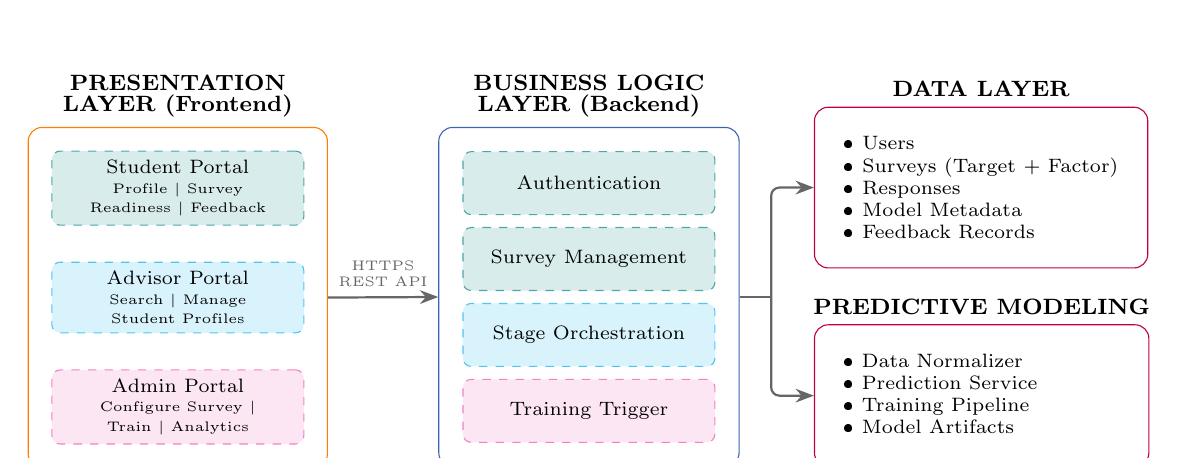
\begin{tikzpicture}[
    node distance=1.5mm,
    box/.style={draw, dashed, rounded corners=3pt, minimum width=32mm, minimum height=8mm, align=center, font=\scriptsize},
    layer/.style={draw, rounded corners=5pt, inner sep=3mm},
    student/.style={box, draw=teal!70, fill=teal!15},
    advisor/.style={box, draw=cyan!70, fill=cyan!15},
    admin/.style={box, draw=magenta!50, fill=magenta!10},
    lbl/.style={font=\footnotesize\bfseries, align=center},
    >=Stealth
]

\node[student] (auth) {Authentication};
\node[student, below=of auth] (surv) {Survey Management};
\node[advisor, below=of surv] (stage) {Stage Orchestration};
\node[admin, below=of stage] (train) {Training Trigger};

\begin{scope}[on background layer]
\node[layer, draw=dblue, fit=(auth)(surv)(stage)(train), label={[lbl]above:BUSINESS LOGIC\\[-2pt]LAYER (Backend)}] (biz) {};
\end{scope}

\path let \p1=(biz.north), \p2=(biz.south), \p3=(biz.west) in
    node[layer, draw=orange,
         minimum height={\y1-\y2},
         minimum width=38mm,
         anchor=north east,
         label={[lbl]above:PRESENTATION\\[-2pt]LAYER (Frontend)}] (pres) at ($(\x3,\y1)+(-14mm,0)$) {};

\node[student, anchor=north] at ($(pres.north)+(0,-3mm)$) (sp) {Student Portal\\[-1pt]\tiny Profile \textbar{} Survey\\[-1pt]\tiny Readiness \textbar{} Feedback};
\node[advisor] at (pres.center) (ap) {Advisor Portal\\[-1pt]\tiny Search \textbar{} Manage\\[-1pt]\tiny Student Profiles};
\node[admin, anchor=south] at ($(pres.south)+(0,3mm)$) (adm) {Admin Portal\\[-1pt]\tiny Configure Survey \textbar{} \\[-1pt]\tiny Train \textbar{} Analytics};

\path let \p1=(biz.north east) in
    node[font=\scriptsize, align=left, anchor=north west] (dlist) at ($(\x1,\y1)+(12mm,0)$) {
        \textbullet\ Users\\
        \textbullet\ Surveys (Target + Factor)\\
        \textbullet\ Responses\\
        \textbullet\ Model Metadata\\
        \textbullet\ Feedback Records
    };

\begin{scope}[on background layer]
\node[layer, draw=purple, fit=(dlist), inner sep=2.5mm, label={[lbl]above:DATA LAYER}] (data) {};
\end{scope}

\path let \p1=(data.west), \p2=(data.east), \p3=(biz.south) in
    node[layer, draw=purple, minimum width={\x2-\x1}, minimum height=18mm, anchor=south west, label={[lbl]above:PREDICTIVE MODELING}] (ml) at (\x1,\y3) {};

\node[font=\scriptsize, align=left, anchor=north west] at ($(ml.north west)+(2.5mm,-2.5mm)$) {
    \textbullet\ Data Normalizer\\
    \textbullet\ Prediction Service\\
    \textbullet\ Training Pipeline\\
    \textbullet\ Model Artifacts
};

\draw[->, thick, black!60] (pres.east) -- (biz.west) node[midway, above, font=\tiny, align=center] {HTTPS\\REST API};
\coordinate (split) at ($(biz.east)+(4mm,0)$);
\draw[thick, black!60] (biz.east) -- (split);
\draw[->, thick, black!60, rounded corners=3pt] (split) |- (data.west);
\draw[->, thick, black!60, rounded corners=3pt] (split) |- (ml.west);

\end{tikzpicture}
}\end{figure}

\begin{quote}\footnotesize
\textit{Diagram text changes:} \DIFadd{ACOSUS} \DIFadd{system} \DIFadd{architecture.} \DIFadd{Four} \DIFadd{layers} \DIFadd{separate} \DIFadd{presentation,} \DIFadd{business} \DIFadd{logic,} \DIFadd{data} \DIFadd{persistence,} \DIFadd{and} \DIFadd{predictive} \DIFadd{modeling,} \DIFadd{enabling} \DIFadd{independent} \DIFadd{scaling} \DIFadd{and} \DIFadd{clear} \DIFadd{separation} \DIFadd{of} \DIFadd{responsibilities.}; Authentication; Survey Management; Stage Orchestration; Training Trigger; Student Portal [-1pt] Profile | Survey [-1pt] \DIFdel{Prediction} \DIFadd{Readiness} | Feedback; Advisor Portal [-1pt] Search | Manage [-1pt] Student Profiles; Admin Portal [-1pt] Configure Survey | [-1pt] Train | Analytics
\end{quote}

\subsection{Dual-Survey Architecture}\label{subsec:dualsurvey}

\DIFdel{This} \DIFadd{In} \DIFdel{section} \DIFadd{this} \DIFdel{introduces} \DIFadd{paper,} \textbf{\DIFadd{student} \DIFadd{success}} \DIFadd{refers} \DIFadd{to} \DIFadd{persistence} \DIFadd{after} \DIFadd{transfer,} \DIFadd{satisfactory} \DIFadd{academic} \DIFadd{progress} \DIFadd{and} \DIFadd{credit} \DIFadd{accumulation,} \DIFadd{and} \DIFadd{eventual} \DIFadd{bachelor's} \DIFadd{degree} \DIFadd{completion.} \DIFadd{These} \DIFadd{outcomes} \DIFadd{require} \DIFadd{longitudinal} \DIFadd{institutional} \DIFadd{records} \DIFadd{and} \DIFadd{were} \DIFadd{not} \DIFadd{observed} \DIFadd{in} the \DIFdel{terms} \DIFadd{pilot.} \DIFdel{used} \DIFadd{The} \DIFdel{throughout} \DIFadd{Target} \DIFdel{the} \DIFadd{Survey} \DIFdel{paper.} \DIFadd{instead} \DIFdel{ACOSUS} \DIFadd{provides} \DIFdel{treats} \DIFadd{a} \DIFdel{transfer} \DIFadd{proximal,} \DIFadd{self-reported} \textbf{\DIFadd{readiness} \DIFadd{measure}} \DIFadd{based} \DIFadd{on} \DIFadd{students}' \DIFadd{reports} \DIFadd{of} \DIFadd{academic} \DIFadd{confidence,} \DIFadd{commitment,} \DIFadd{time} \DIFadd{management,} \DIFadd{and} \DIFadd{related} \DIFadd{constructs} \DIFadd{at} \DIFadd{one} \DIFadd{point} \DIFadd{in} \DIFadd{time.} \DIFadd{The} \DIFadd{measure} \DIFadd{is} \DIFadd{not} \DIFadd{an} \DIFadd{observed} \DIFadd{success} \DIFadd{outcome} \DIFadd{or} \DIFadd{evidence} \DIFadd{that} \DIFadd{a} student \DIFdel{success} \DIFadd{will} \DIFdel{prediction} \DIFadd{persist} \DIFdel{as} \DIFadd{or} \DIFdel{a} \DIFdel{supervised} \DIFdel{learning} \DIFdel{problem} \DIFdel{in} \DIFdel{which} \DIFdel{an} \DIFdel{outcome} \DIFdel{is} \DIFdel{predicted} \DIFdel{from} \DIFdel{a} \DIFdel{set} \DIFdel{of} \DIFdel{input} \DIFdel{variables.} \DIFdel{Because} \DIFdel{the} \DIFdel{platform} \DIFdel{separates} \DIFdel{what} \DIFdel{is} \DIFdel{being} \DIFdel{predicted} \DIFdel{from} \DIFdel{the} \DIFdel{information} \DIFdel{used} \DIFdel{to} \DIFdel{make} \DIFdel{that} \DIFdel{prediction,} \DIFdel{three} \DIFdel{terms} \DIFdel{are} \DIFdel{central} \DIFdel{to} \DIFdel{the} \DIFdel{design:} \DIFadd{graduate.}

\DIFadd{This} \DIFadd{section} \DIFadd{introduces} \DIFadd{the} \DIFadd{terms} \DIFadd{used} \DIFadd{throughout} \DIFadd{the} \DIFadd{paper.} \DIFadd{ACOSUS} \DIFadd{treats} \DIFadd{future} \DIFadd{transfer-student} \DIFadd{outcome} \DIFadd{prediction} \DIFadd{as} \DIFadd{a} \DIFadd{supervised} \DIFadd{learning} \DIFadd{problem} \DIFadd{in} \DIFadd{which} \DIFadd{an} \DIFadd{outcome} \DIFadd{is} \DIFadd{predicted} \DIFadd{from} \DIFadd{a} \DIFadd{set} \DIFadd{of} \DIFadd{input} \DIFadd{variables.} \DIFadd{Because} \DIFadd{the} \DIFadd{platform} \DIFadd{separates} \DIFadd{what} \DIFadd{is} \DIFadd{being} \DIFadd{measured} \DIFadd{from} \DIFadd{the} \DIFadd{information} \DIFadd{used} \DIFadd{to} \DIFadd{estimate} \DIFadd{it,} \DIFadd{three} \DIFadd{terms} \DIFadd{are} \DIFadd{central} \DIFadd{to} \DIFadd{the} \DIFadd{design:}

\begin{itemize}
    \item \textbf{Target Survey / \DIFdel{Outcome} \DIFadd{Readiness} \DIFadd{Measure} ($Y$)}: The survey instrument that \DIFdel{measures} \DIFdel{what} \DIFdel{we} \DIFdel{want} \DIFdel{to} \DIFdel{predict,} \DIFdel{namely} \DIFadd{produces} the \DIFdel{student's} \DIFadd{current} \DIFdel{likelihood} \DIFadd{proximal,} \DIFdel{of} \DIFadd{self-reported} \DIFdel{academic} \DIFdel{success.} \DIFadd{measure.} In machine learning terminology, this is the \emph{label} or \emph{dependent variable}.
    \item \textbf{Factor Survey / Predictors ($X$)}: The survey instruments that collect information used to make predictions, including academic background, financial circumstances, and logistical constraints. In machine learning terminology, these are \emph{features} or \emph{independent variables}.
    \item \textbf{Constructs}: Psychological or educational concepts (e.g., self-efficacy, institutional commitment) that we operationalize through survey questions. A single Factor Survey may measure multiple constructs.
\end{itemize}

These definitions matter because many of the factors that shape transfer success do not map cleanly onto the information universities already store. Variables such as credit articulation outcomes, transfer shock, belonging, and financial precarity are rarely captured in standard institutional systems \parencite{nguyen2025school}. Advisors also often lack one place to access the information they need; prior work shows that they spend substantial time gathering student data from multiple sources before they can offer useful guidance \parencite{preposttransfer2014}. ACOSUS addresses both issues through a dual-survey architecture that supports prediction while also consolidating advisor-facing information.

Prior research identifies several dimensions \DIFdel{of} \DIFadd{associated} \DIFadd{with} transfer success, including academic self-efficacy, institutional commitment, social integration, and career clarity \parencite{factoranalysis2023}. Our earlier factor-analysis work grouped related variables into clusters such as academic confidence, time management, financial stability, and support systems \parencite{factoranalysis2023}. Building on those findings, \DIFadd{in} ACOSUS \DIFdel{treats} \DIFadd{the} ``\DIFdel{success}\DIFdel{''} \DIFadd{readiness} \DIFdel{as} \DIFadd{measure}\DIFadd{``} \DIFdel{a} \DIFadd{summarizes} \DIFdel{student's} \DIFadd{how} \DIFdel{likelihood} \DIFadd{students} \DIFdel{of} \DIFadd{assess} \DIFdel{doing} \DIFadd{their} \DIFdel{well} \DIFadd{present} \DIFadd{preparation} across these \DIFdel{dimensions} \DIFadd{dimensions,} \DIFdel{and} \DIFdel{``}\DIFdel{factors}\DIFdel{''} \DIFdel{as} \DIFadd{while} the \DIFadd{Factor} \DIFadd{Surveys} \DIFadd{capture} conditions that \DIFadd{may} affect \DIFdel{that} \DIFadd{future} \DIFdel{likelihood.} \DIFadd{outcomes.}

ACOSUS implements this framework through a Dual-Survey Architecture that separates \DIFdel{outcome} \DIFadd{readiness} \DIFdel{collection} \DIFadd{measurement} from predictor collection (Figure~\ref{fig:dualsurvey}). \textbf{Target Surveys} (measuring $Y$) \DIFdel{capture} \DIFdel{success} \DIFdel{through} \DIFadd{support} two \DIFdel{supported} modes: (1) a single direct self-assessment question where students rate their \DIFdel{success} \DIFadd{readiness} on a 0--100 scale, or (2) a multi-question instrument measuring \DIFdel{constructs} \DIFdel{such} \DIFdel{as} academic confidence, commitment, time management self-efficacy, \DIFdel{and} career motivation, \DIFadd{and} \DIFadd{related} \DIFadd{constructs,} which are aggregated \DIFdel{into} \DIFdel{a} \DIFdel{single} \DIFdel{score} \DIFdel{via} \DIFadd{through} weighted calculation. \textbf{Factor Surveys} (measuring $X$) collect \DIFdel{the} predictor variables \DIFdel{used} \DIFdel{for} \DIFdel{prediction,} organized into categories such as academic background, financial circumstances, logistical constraints, and prior interests or experiences.

Beyond their role as predictor vectors for the AI model, Factor Surveys also help advisors by standardizing the collection of transfer-specific information that would otherwise be gathered through lengthy and inconsistent interviews. Every transfer student answers the same set of questions, which supports cohort-level comparison and reduces the chance that important risk factors will be missed. Survey responses are immediately available in the advisor dashboard, which reduces the need to search through emails, notes, or follow-up conversations.

The architecture also supports flexible study designs through \textbf{survey linkage}, that is, explicit associations between Target and Factor Surveys. This makes it possible to compare different predictor sets, add new factors over time, and customize the system for different cohorts without changing the core infrastructure. Once these surveys are linked and deployed, the next step is to transform raw responses into model-ready inputs. We return to the linkage mechanism from an implementation perspective when discussing configuration flexibility later in the paper.

\begin{figure}[htbp]
\centering
\caption{Dual-Survey Architecture. Target Surveys collect the outcome ($Y$), Factor Surveys collect predictors ($X$). Dashed lines show linkage relationships enabling flexible study configurations.}
\label{fig:dualsurvey}
\resizebox{0.72\textwidth}{!}{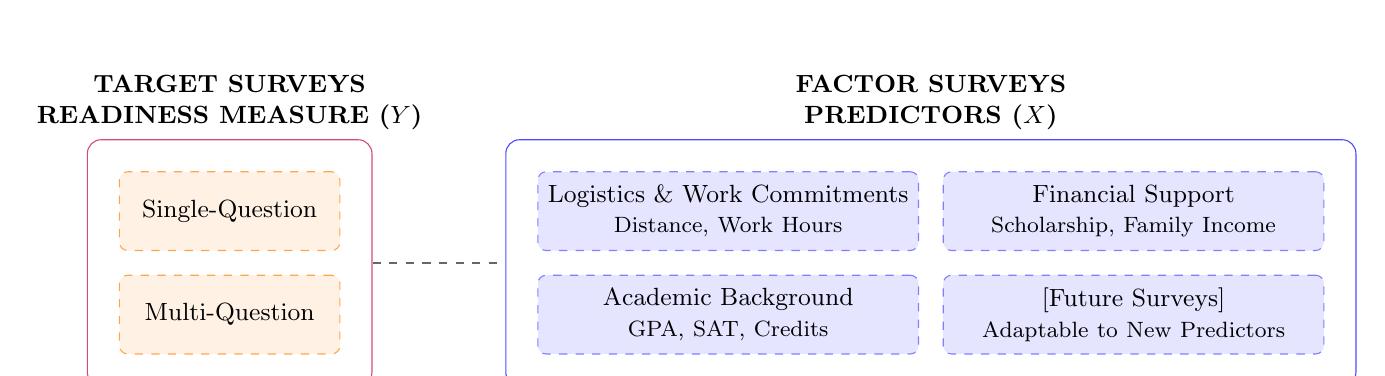
\begin{tikzpicture}[
  box/.style={draw,dashed,rounded corners=3pt,align=center,font=\small},
  target/.style={box,draw=orange!70,fill=orange!10,minimum width=28mm,minimum height=10mm},
  factor/.style={box,draw=blue!50,fill=blue!10,minimum width=48mm,minimum height=10mm,text width=46mm},
  container/.style={draw,rounded corners=5pt,inner sep=4mm}
]
\node[target] (sq) {Single-Question};
\node[target,below=3mm of sq] (mq) {Multi-Question};
\node[container,draw=purple!70,fit=(sq)(mq),label={[font=\small\bfseries,align=center]above:TARGET SURVEYS\\READINESS MEASURE ($Y$)}] (tbox) {};
\node[factor,right=25mm of sq] (lc) {Logistics \& Work Commitments\\\footnotesize Distance, Work Hours};
\node[factor,right=3mm of lc] (fs) {Financial Support\\\footnotesize Scholarship, Family Income};
\node[factor,below=3mm of lc] (ab) {Academic Background\\\footnotesize GPA, SAT, Credits};
\node[factor,right=3mm of ab] (fu) {[Future Surveys]\\\footnotesize Adaptable to New Predictors};
\node[container,draw=blue!70,fit=(lc)(fs)(ab)(fu),label={[font=\small\bfseries,align=center]above:FACTOR SURVEYS\\PREDICTORS ($X$)}] (fbox) {};

\draw[black!60,dashed,thick] (tbox.east) -- (fbox.west);
\end{tikzpicture}
}\end{figure}

\begin{quote}\footnotesize
\textit{Diagram text changes:} \DIFadd{Dual-Survey} \DIFadd{Architecture.} \DIFadd{Target} \DIFadd{Surveys} \DIFadd{collect} \DIFadd{the} \DIFadd{outcome} ($\DIFadd{Y}$), \DIFadd{Factor} \DIFadd{Surveys} \DIFadd{collect} \DIFadd{predictors} ($\DIFadd{X}$). \DIFadd{Dashed} \DIFadd{lines} \DIFadd{show} \DIFadd{linkage} \DIFadd{relationships} \DIFadd{enabling} \DIFadd{flexible} \DIFadd{study} \DIFadd{configurations.}; Single-Question; Multi-Question; Logistics \& \DIFdel{Commitment} \DIFadd{Work} \DIFadd{Commitments} Distance, Work Hours; Financial Support Scholarship, Family Income; Academic Background GPA, SAT, Credits; [Future Surveys] Adaptable to New Predictors
\end{quote}

\subsection{Survey Data Processing}\label{subsec:dataprocessing}

The Target and Factor Survey instruments convert student responses into feature vectors for predictive modeling, following the pipeline shown in Figure~\ref{fig:processing}. Each question corresponds to a success-related factor identified in prior research. Our earlier factor-analysis work linked observable indicators such as scholarship status and commute distance to broader constructs such as financial stability and institutional commitment \parencite{factoranalysis2023}. The purpose of this stage is to move from survey design to a consistent numerical representation that later modeling stages can use.

\subsubsection{Priority Weighting}

Not all factors contribute equally to student success. Without an explicit weighting mechanism, a \DIFdel{prediction} \DIFadd{readiness} \DIFdel{model} \DIFadd{calculation} would treat every survey question as equally informative, giving commute distance the same influence as academic self-efficacy. \DIFdel{This} \DIFdel{contradicts} \DIFdel{retention} \DIFadd{Prior} research \DIFdel{showing} \DIFadd{suggests} that \DIFdel{certain} \DIFadd{some} constructs \DIFdel{are} \DIFadd{may} \DIFdel{substantially} \DIFadd{be} \DIFdel{stronger} \DIFadd{more} \DIFdel{predictors} \DIFadd{strongly} \DIFdel{of} \DIFadd{associated} \DIFadd{with} persistence than logistical variables \parencite{factoranalysis2023}. \DIFdel{A} \DIFadd{An} \DIFdel{flat} \DIFadd{equal-weighting} \DIFdel{weighting} \DIFadd{scheme} would also make the \DIFdel{system} \DIFadd{calculation} less interpretable for advisors, who need to understand \DIFdel{why} \DIFadd{how} a particular \DIFdel{risk} score was generated. Prior research \DIFdel{consistently} identifies \DIFdel{some} \DIFadd{academic,} \DIFdel{variables} \DIFadd{financial,} \DIFdel{academic} \DIFdel{self-efficacy,} \DIFdel{financial} \DIFdel{stability,} \DIFadd{institutional,} and \DIFdel{institutional} \DIFadd{logistical} \DIFdel{fit,} \DIFadd{factors} \DIFdel{for} \DIFadd{that} \DIFdel{example} \DIFadd{can} \DIFdel{as} \DIFadd{shape} \DIFdel{more} \DIFadd{transfer} \DIFdel{predictive} \DIFadd{experiences} \DIFdel{than} \DIFdel{others} \DIFdelcite{\parencite{computingtransfer2024}} \DIFaddcite{\parencite{factoranalysis2023,computingtransfer2024}}. ACOSUS accounts for \DIFdel{this} \DIFadd{these} \DIFadd{differences} through \textbf{priority scores}. \DIFdel{These} \DIFadd{The} \DIFadd{current} scores are \DIFdel{based} \DIFadd{literature-informed} \DIFdel{on} \DIFadd{starting} \DIFdel{empirical} \DIFdel{evidence} \DIFdel{such} \DIFdel{as} \DIFdel{effect} \DIFdel{sizes} \DIFadd{values} and \DIFdel{factor} \DIFadd{design} \DIFdel{loadings} \DIFadd{choices,} \DIFdel{from} \DIFadd{not} \DIFdel{prior} \DIFadd{coefficients} \DIFdel{studies,} \DIFadd{estimated} \DIFdel{and} \DIFadd{or} \DIFdel{they} \DIFadd{validated} \DIFadd{using} \DIFadd{ACOSUS} \DIFadd{longitudinal} \DIFadd{outcomes.} \DIFadd{They} can be adjusted as advisor feedback \DIFdel{clarifies} \DIFadd{and} \DIFadd{institutional} \DIFadd{evidence} \DIFadd{clarify} which factors \DIFdel{matter} \DIFadd{are} most \DIFadd{relevant} in a \DIFdel{given} \DIFdel{institutional} \DIFadd{particular} context (Table~\ref{tab:priority}).

The priority-weighted aggregation follows a straightforward formulation. For a survey with $n$ questions, where question $i$ has priority score $p_i$, the student selects an option with weightage $w_i^{\text{selected}}$ from a maximum possible $w_i^{\text{max}}$:

\begin{equation}
S = \frac{\sum_{i=1}^{n} \left(\frac{w_i^{\text{selected}}}{w_i^{\text{max}}} \times p_i\right)}{\sum_{i=1}^{n} p_i}
\label{eq:priority}
\end{equation}

This yields a normalized score in $[0, 1]$ that reflects both the selected response and the \DIFdel{importance} \DIFadd{priority} of the corresponding question. \DIFdel{We} \DIFadd{A} \DIFdel{then} \DIFadd{bounded} \DIFdel{apply} \DIFadd{calibration} \DIFadd{step} \DIFadd{converts} \DIFadd{the} \DIFadd{result} \DIFadd{to} \DIFadd{the} \DIFadd{readiness-score} \DIFadd{scale.} \DIFadd{The} \DIFadd{same} \DIFadd{priority-weighted} \DIFadd{calculation} \DIFadd{can} \DIFadd{aggregate} a \DIFdel{logistic} \DIFadd{multi-question} \DIFdel{calibration} \DIFadd{Target} \DIFdel{curve} \DIFadd{Survey} \DIFdel{to} \DIFadd{and} \DIFdel{reduce} \DIFadd{provide} \DIFdel{overconfident} \DIFadd{a} \DIFdel{predictions} \DIFadd{transparent} \DIFdel{at} \DIFadd{summary} \DIFdel{the} \DIFadd{of} \DIFdel{extremes.} \DIFadd{Factor} \DIFadd{Survey} \DIFadd{responses} \DIFadd{for} \DIFadd{later} \DIFadd{exploratory} \DIFadd{modeling.}

\begin{table}[htbp]

\caption{\DIFdel{Example} \DIFadd{Literature-informed} priority \DIFdel{score} \DIFadd{structure} \DIFdel{assignments} \DIFadd{used} \DIFdel{based} \DIFadd{in} \DIFdel{on} \DIFadd{the} \DIFdel{literature-informed} \DIFdel{importance.} \DIFadd{prototype}}
\label{tab:priority}
 \centering
\begin{tabularx}{\textwidth}{@{}>{\hsize=.70\hsize\linewidth=\hsize}Y>{\hsize=1.70\hsize\linewidth=\hsize}Y>{\hsize=.60\hsize\linewidth=\hsize}Y@{}}
\toprule
\textbf{Factor Category} & \textbf{\DIFdel{Example} \DIFadd{Question} \DIFdel{Question} \DIFadd{Topics}} & \textbf{\DIFdel{Priority}  \DIFdel{Rationale} \DIFadd{Emphasis}} \\
\midrule
Academic          \DIFdel{Self-Efficacy} \DIFadd{background} & \DIFdel{How} \DIFadd{GPA,} \DIFdel{confident} \DIFadd{prior} \DIFdel{in} \DIFadd{academic} \DIFdel{your} \DIFadd{preparation,} \DIFdel{ability} \DIFadd{completed} \DIFdel{to} \DIFadd{credits,} \DIFdel{succeed?} \DIFadd{and} \DIFadd{course} \DIFadd{load} & \DIFdel{9}  \DIFdel{Strong} \DIFdel{predictor} \DIFdelcite{\parencite{bandura1997}} \DIFadd{Higher} \\
\addlinespace[2pt]
\DIFdel{Financial} \DIFadd{Program} \DIFdel{Stability} \DIFadd{timeline} & \DIFdel{Expected} \DIFadd{Program} \DIFdel{financial} \DIFadd{start} \DIFdel{stress} \DIFadd{and} \DIFdel{impact?} \DIFadd{expected} \DIFadd{completion} & \DIFdel{8}  \DIFdel{Affects} \DIFdel{retention} \DIFdelcite{\parencite{socialcognitive2022}} \DIFadd{Higher} \\
\addlinespace[2pt]
\DIFdel{Institutional} \DIFadd{Financial} \DIFdel{Commitment} \DIFadd{support} & \DIFdel{How} \DIFadd{Scholarship} \DIFdel{committed} \DIFadd{and} \DIFdel{to} \DIFadd{family} \DIFdel{completing} \DIFdel{this} \DIFdel{program?} \DIFadd{support} & \DIFdel{9}  \DIFdel{Persistence} \DIFdel{indicator} \DIFdelcite{\parencite{tinto1993}} \DIFadd{Lower} \\
\addlinespace[2pt]
Logistics \DIFadd{and} \DIFadd{commitments} & Commute \DIFdel{distance} \DIFadd{and} \DIFadd{work} \DIFadd{commitments} & \DIFadd{Moderate} to higher \\
\addlinespace[2pt]
Interests and experience & \DIFdel{6} \DIFadd{Career} \DIFadd{goals,} \DIFadd{course} \DIFadd{interest,} \DIFadd{and} \DIFadd{prior} \DIFadd{experience} & \DIFdel{Practical} \DIFadd{Varies} \DIFdel{barrier} \DIFadd{by} \DIFadd{factor} \\
\bottomrule
 \end{tabularx}
\end{table}

\DIFdel{These} \DIFadd{To} \DIFdel{priority} \DIFadd{show} \DIFdel{weights} \DIFadd{how} \DIFdel{also} \DIFadd{the} \DIFdel{remain} \DIFadd{starting} \DIFdel{useful} \DIFadd{priorities} \DIFadd{affect} \DIFadd{the} \DIFadd{result,} \DIFadd{we} \DIFadd{recalculated} \DIFadd{scores} \DIFadd{for} \DIFadd{the} \DIFadd{available} \DIFadd{deidentified} \DIFadd{pilot} \DIFadd{profiles} \DIFadd{under} \DIFadd{three} \DIFadd{alternative} \DIFadd{scenarios.} \DIFadd{The} \DIFadd{analysis} \DIFadd{used} \DIFadd{the} \DIFadd{factor} \DIFadd{responses} \DIFadd{represented} \DIFadd{across} \DIFadd{those} \DIFadd{profiles} \DIFadd{and} \DIFadd{the} \DIFadd{same} \DIFadd{priority-weighted} \DIFadd{calculation} in \DIFdel{later} \DIFadd{each} \DIFdel{modeling} \DIFadd{scenario.}
\DIFdel{stages.} \DIFdel{When} \DIFdel{ACOSUS} \DIFdel{moves} \DIFdel{to} \DIFdel{probabilistic} \DIFdel{methods,} \DIFadd{Table}~\DIFaddcite{\ref{tab:sensitivity} }\DIFadd{reports} the \DIFdel{weights} \DIFadd{resulting} \DIFdel{can} \DIFadd{sensitivity} \DIFdel{be} \DIFdel{used} \DIFdel{as} \DIFdel{informative} \DIFdel{priors} \DIFdel{or} \DIFdel{as} \DIFdel{a} \DIFdel{principled} \DIFdel{starting} \DIFdel{point,} \DIFdel{so} \DIFdel{that} \DIFdel{features} \DIFdel{with} \DIFdel{higher} \DIFdel{priorities} \DIFdel{have} \DIFdel{greater} \DIFdel{initial} \DIFdel{influence} \DIFdel{before} \DIFdel{the} \DIFdel{model} \DIFdel{updates} \DIFdel{them} \DIFdel{using} \DIFdel{observed} \DIFdel{data.} \DIFdel{This} \DIFdel{preserves} \DIFdel{a} \DIFdel{link} \DIFdel{between} \DIFdel{expert} \DIFdel{knowledge} \DIFdel{and} \DIFdel{learned} \DIFdel{parameters.} \DIFdel{The} \DIFdel{next} \DIFdel{step} \DIFdel{in} \DIFdel{processing} \DIFdel{is} \DIFdel{to} \DIFdel{ensure} \DIFdel{that} \DIFdel{different} \DIFdel{kinds} \DIFdel{of} \DIFdel{survey} \DIFdel{responses} \DIFdel{are} \DIFdel{normalized} \DIFdel{appropriately.} \DIFadd{comparison.}

\begin{table}[htbp]
\caption{Priority-weight sensitivity across the available pilot profiles}
\label{tab:sensitivity}
\centering
\begin{tabularx}{\textwidth}{@{}Yrrrr@{}}
\toprule
\textbf{Scenario} & \textbf{Mean} & \textbf{Range} & \textbf{Mean $|\Delta|$} & \textbf{Max $|\Delta|$} \\
\midrule
Baseline priorities & 82.27 & 72.25--91.38 & 0.00 & 0.00 \\
Equal weighting & 81.10 & 67.82--91.16 & 1.77 & 5.24 \\
Double academic priorities & 81.35 & 71.27--91.92 & 1.22 & 2.63 \\
Double support/logistics priorities & 81.76 & 70.35--91.22 & 1.23 & 3.21 \\
\bottomrule
\end{tabularx}
\end{table}

\DIFadd{The} \DIFadd{comparison} \DIFadd{shows} \DIFadd{how} \DIFadd{different} \DIFadd{priority} \DIFadd{configurations} \DIFadd{change} \DIFadd{the} \DIFadd{calculated} \DIFadd{readiness} \DIFadd{scores.} \DIFadd{Across} \DIFadd{the} \DIFadd{ten} \DIFadd{profiles,} \DIFadd{the} \DIFadd{tested} \DIFadd{alternatives} \DIFadd{produced} \DIFadd{limited} \DIFadd{average} \DIFadd{movement} \DIFadd{from} \DIFadd{the} \DIFadd{baseline.} \DIFadd{Under} \DIFadd{equal} \DIFadd{weighting,} \DIFadd{the} \DIFadd{mean} \DIFadd{absolute} \DIFadd{difference} \DIFadd{was} \DIFadd{1.}\DIFadd{77} \DIFadd{points,} \DIFadd{while} \DIFadd{the} \DIFadd{largest} \DIFadd{difference} \DIFadd{was} \DIFadd{5.}\DIFadd{24} \DIFadd{points} \DIFadd{for} \DIFadd{one} \DIFadd{profile,} \DIFadd{whose} \DIFadd{score} \DIFadd{decreased} \DIFadd{from} \DIFadd{78.}\DIFadd{11} \DIFadd{to} \DIFadd{72.}\DIFadd{87.} \DIFadd{Because} \DIFadd{the} \DIFadd{priorities} \DIFadd{are} \DIFadd{prototype} \DIFadd{configuration} \DIFadd{values} \DIFadd{and} \DIFadd{the} \DIFadd{scores} \DIFadd{are} \DIFadd{deterministic} \DIFadd{survey} \DIFadd{composites,} \DIFadd{these} \DIFadd{results} \DIFadd{describe} \DIFadd{sensitivity} \DIFadd{within} \DIFadd{this} \DIFadd{small} \DIFadd{set;} \DIFadd{they} \DIFadd{do} \DIFadd{not} \DIFadd{identify} \DIFadd{optimal} \DIFadd{priorities,} \DIFadd{validate} \DIFadd{the} \DIFadd{readiness} \DIFadd{measure} \DIFadd{as} \DIFadd{a} \DIFadd{predictor} \DIFadd{of} \DIFadd{student} \DIFadd{success,} \DIFadd{or} \DIFadd{evaluate} \DIFadd{fairness.} \DIFadd{The} \DIFadd{priorities} \DIFadd{can} \DIFadd{be} \DIFadd{re-estimated} \DIFadd{and} \DIFadd{updated} \DIFadd{as} \DIFadd{larger} \DIFadd{samples} \DIFadd{and} \DIFadd{longitudinal} \DIFadd{persistence,} \DIFadd{credit-accumulation,} \DIFadd{and} \DIFadd{completion} \DIFadd{outcomes} \DIFadd{become} \DIFadd{available.}

\DIFadd{These} \DIFadd{priority} \DIFadd{weights} \DIFadd{can} \DIFadd{also} \DIFadd{serve} \DIFadd{as} \DIFadd{informative} \DIFadd{priors} \DIFadd{or} \DIFadd{principled} \DIFadd{starting} \DIFadd{points} \DIFadd{in} \DIFadd{later} \DIFadd{probabilistic} \DIFadd{models,} \DIFadd{allowing} \DIFadd{observed} \DIFadd{data} \DIFadd{to} \DIFadd{update} \DIFadd{their} \DIFadd{influence.} \DIFadd{This} \DIFadd{preserves} \DIFadd{a} \DIFadd{link} \DIFadd{between} \DIFadd{prior} \DIFadd{research,} \DIFadd{transparent} \DIFadd{design} \DIFadd{choices,} \DIFadd{and} \DIFadd{learned} \DIFadd{parameters} \DIFadd{without} \DIFadd{treating} \DIFadd{the} \DIFadd{starting} \DIFadd{values} \DIFadd{as} \DIFadd{established} \DIFadd{effects.} \DIFadd{The} \DIFadd{next} \DIFadd{step} \DIFadd{in} \DIFadd{processing} \DIFadd{is} \DIFadd{to} \DIFadd{ensure} \DIFadd{that} \DIFadd{different} \DIFadd{kinds} \DIFadd{of} \DIFadd{survey} \DIFadd{responses} \DIFadd{are} \DIFadd{normalized} \DIFadd{appropriately.}

\subsubsection{Data Type Handling}

Survey responses include different data types, and each type requires an appropriate normalization step before modeling, as summarized in Table~\ref{tab:normalization}. The distinction between \textbf{ordinal} and \textbf{cardinal} data is especially important: ordinal responses (e.g., ``Not confident'' $<$ ``Somewhat confident'' $<$ ``Very confident'') have a meaningful order, whereas cardinal responses (e.g., career aspiration categories) do not imply ranking.

\begin{table}[htbp]
\centering
\caption{Normalization strategies for different data \DIFdel{types.} \DIFadd{types}}
\label{tab:normalization}
 \begin{tabularx}{\textwidth}{@{}llY@{}}
\toprule
\textbf{Data Type} & \textbf{Example} & \textbf{Normalization Method} \\
\midrule
Ordinal & GPA range: ``3.0--3.5'' & Direct option weightage (e.g., 8/10) \\
Cardinal & Career: ``Industry/Corporate'' & Equal weightage or domain-specific mapping \\
Continuous & SAT score: 1250 & Min-max scaling: $(x - \min)/(\max - \min)$ \\
\bottomrule
 \end{tabularx}
\end{table}

This type-aware processing preserves the meaning of the responses during feature engineering: ordinal relationships remain ordered, nominal categories are not treated as ranked, and continuous values are scaled appropriately. With this processing in place, ACOSUS can pass standardized inputs to the prediction pipeline. The next subsection explains how that pipeline is designed for settings where only a small amount of institutional data is available at first.

\begin{figure}[htbp]
\centering
\caption{Survey data processing pipeline. Raw responses undergo priority weighting and type-aware normalization to produce standardized feature vectors for model ingestion.}
\label{fig:processing}
\resizebox{0.80\textwidth}{!}{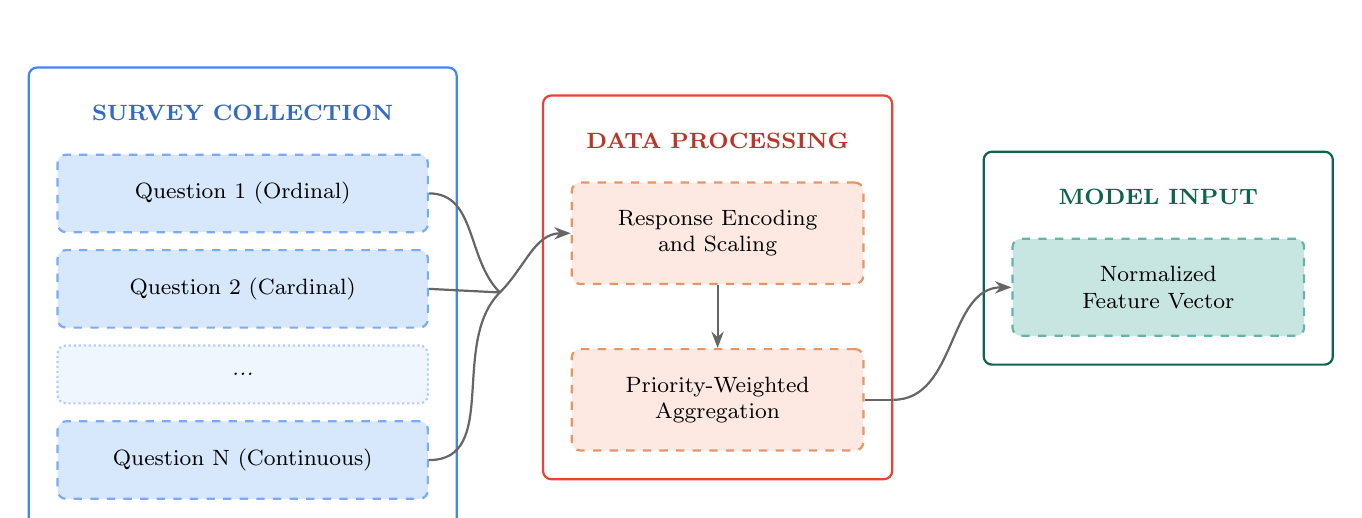
\begin{tikzpicture}[
    node distance=0.35cm,
    inner/.style={rectangle, dashed, thick, rounded corners=3pt, align=center, inner sep=10pt, font=\footnotesize},
    outer/.style={rectangle, thick, rounded corners=3pt, inner sep=6pt},
    arrow/.style={-{Stealth[scale=0.9]}, black!60, thick, rounded corners=6pt},
    arrowline/.style={black!60, thick, rounded corners=6pt}
]

\node[inner, fill=surveyboxfill, draw=surveyblue!70, text width=4cm, minimum height=0.5cm] (q1) {Question 1 (Ordinal)};
\node[inner, fill=surveyboxfill, draw=surveyblue!70, text width=4cm, minimum height=.5cm, below=0.2cm of q1] (q2) {Question 2 (Cardinal)};
\node[inner, fill=surveyboxfill!40, draw=surveyblue!40, densely dotted, text width=4cm, minimum height=.5cm, below=0.2cm of q2] (qdots) {\textit{...}};
\node[inner, fill=surveyboxfill, draw=surveyblue!70, text width=4cm, minimum height=0.5cm, below=0.2cm of qdots] (qn) {Question N (Continuous)};

\node[above=0.3cm of q1, font=\footnotesize\bfseries, text=surveyblue!80!black] (survey-title) {SURVEY COLLECTION};
\node[outer, draw=surveyblue, fit=(survey-title)(q1)(q2)(qdots)(qn), inner sep=10pt] (survey-box) {};

\node[inner, fill=processboxfill, draw=processboxborder, text width=3cm, minimum height=1cm, right=1.8cm of q1.east |- q1.south east] (normalize) {Response Encoding\\and Scaling};
\node[inner, fill=processboxfill, draw=processboxborder, text width=3cm, minimum height=1cm, below=0.8cm of normalize] (priority) {Priority-Weighted\\Aggregation};

\node[above=0.3cm of normalize, font=\footnotesize\bfseries, text=processorange!80!black] (process-title) {DATA PROCESSING};
\node[outer, draw=processorange, fit=(process-title)(normalize)(priority), inner sep=10pt] (process-box) {};

\path (normalize.center) -- (priority.center) coordinate[midway] (process-center);
\node[inner, fill=modelboxfill, draw=modelboxborder, text width=3cm, minimum height=1cm, right=1.5cm of process-box.east, anchor=west] (feature) {Normalized\\Feature Vector};

\node[above=0.3cm of feature, font=\footnotesize\bfseries, text=modelgreen] (model-title) {MODEL INPUT};
\node[outer, draw=modelgreen, fit=(model-title)(feature), inner sep=10pt] (model-box) {};

\coordinate (merge-point) at ($(survey-box.east)!0.5!(process-box.west)$ |- q2);

\draw[arrowline] (q1.east) to[out=0, in=135] (merge-point);
\draw[arrowline] (q2.east) -- (merge-point);
\draw[arrowline] (qn.east) to[out=0, in=-135] (merge-point);
\draw[arrow] (merge-point) to[out=45, in=180] (normalize.west);

\draw[arrow] (normalize.south) -- (priority.north);

\draw[arrowline] (priority.east) -- (process-box.east |- priority.east);
\draw[arrow] (process-box.east |- priority.east) to[out=0, in=180] (feature.west);

\end{tikzpicture}
}
\end{figure}

\begin{quote}\footnotesize
\textit{Diagram text changes:} \DIFadd{Survey} \DIFadd{data} \DIFadd{processing} \DIFadd{pipeline.} \DIFadd{Raw} \DIFadd{responses} \DIFadd{undergo} \DIFadd{priority} \DIFadd{weighting} \DIFadd{and} \DIFadd{type-aware} \DIFadd{normalization} \DIFadd{to} \DIFadd{produce} \DIFadd{standardized} \DIFadd{feature} \DIFadd{vectors} \DIFadd{for} \DIFadd{model} \DIFadd{ingestion.}; Question 1 (Ordinal); Question 2 (Cardinal); \textit{...}; Question N (Continuous); SURVEY COLLECTION; \DIFdel{Priority} \DIFadd{Response} \DIFdel{Weighting;} \DIFadd{Encoding} \DIFdel{Type-Aware} \DIFadd{and} \DIFdel{Normalization;} \DIFadd{Scaling;} \DIFadd{Priority-Weighted} \DIFadd{Aggregation;} DATA PROCESSING; Normalized Feature Vector; MODEL INPUT
\end{quote}

\subsection{Progressive Learning Framework}\label{subsec:progressive}

After survey responses have been standardized, the remaining challenge is how to make use of them when only a small amount of institutional data exists. ACOSUS is designed to work under limited-data conditions from the beginning. Rather than waiting until enough data exist to support prediction, the system provides value from the first student enrollment by giving advisors structured student profiles through standardized surveys. In this way, the early cold-start period still serves a useful advising and data-collection function.

\subsubsection{Three-Stage Pipeline}

As observations accumulate, the system \DIFdel{moves} \DIFadd{is} \DIFadd{designed} \DIFadd{to} \DIFadd{move} through a three-stage pipeline (Figure~\ref{fig:pipeline}):

\textbf{Foundation Stage.} The system focuses on collecting high-quality labeled observations through surveys that capture both \DIFdel{outcomes} \DIFadd{readiness} \DIFadd{measure} and predictors. Once a minimum corpus exists, lightweight methods (e.g., k-nearest neighbors or cosine similarity matching) can generate initial \DIFdel{predictions.} \DIFadd{estimates.} At this stage, data quality matters more than model complexity.

\textbf{Augmentation Stage.} As the corpus grows, the \DIFdel{system} \DIFadd{framework} \DIFdel{uses} \DIFadd{can} \DIFadd{evaluate} generative methods (e.g., SMOTE, generative adversarial networks, or variational autoencoders) \DIFdel{to} \DIFadd{for} \DIFdel{synthesize} \DIFadd{synthesizing} additional training observations. These methods learn from the real data and produce synthetic samples that expand the training set while preserving its main statistical \DIFdel{properties.} \DIFadd{properties;} \DIFadd{the} \DIFadd{resulting} \DIFadd{samples} \DIFadd{must} \DIFadd{also} \DIFadd{be} \DIFadd{evaluated} \DIFadd{for} \DIFadd{fidelity,} \DIFadd{privacy,} \DIFadd{bias,} \DIFadd{and} \DIFadd{utility.}

\textbf{Refinement Stage.} Finally, the \DIFdel{system} \DIFadd{framework} \DIFdel{transitions} \DIFadd{can} \DIFadd{transition} to more advanced non-linear models (e.g., deep neural networks, gradient boosting, or ensemble methods) that can capture complex relationships between features and outcomes.

The framework is modular across all three stages. Any compatible predictive method may be used in the foundation stage, any suitable generative technique may be used for augmentation, and any supervised learning architecture may be used in refinement. This design allows researchers to compare algorithms on their own student populations and to adopt new methods as they become available without redesigning the full system. Because those choices may differ across institutions and studies, the next subsection describes the configuration layer that controls how surveys, stages, and algorithms are connected in practice.

\begin{figure}[htbp]
\centering
\caption{The Three-Stage Progressive Pipeline. Each stage represents a pluggable component that can be substituted with alternative algorithms. The framework progresses from data acquisition through augmentation to refined prediction, with feedback loops enabling continuous improvement.}
\label{fig:pipeline}
\resizebox{\textwidth}{!}{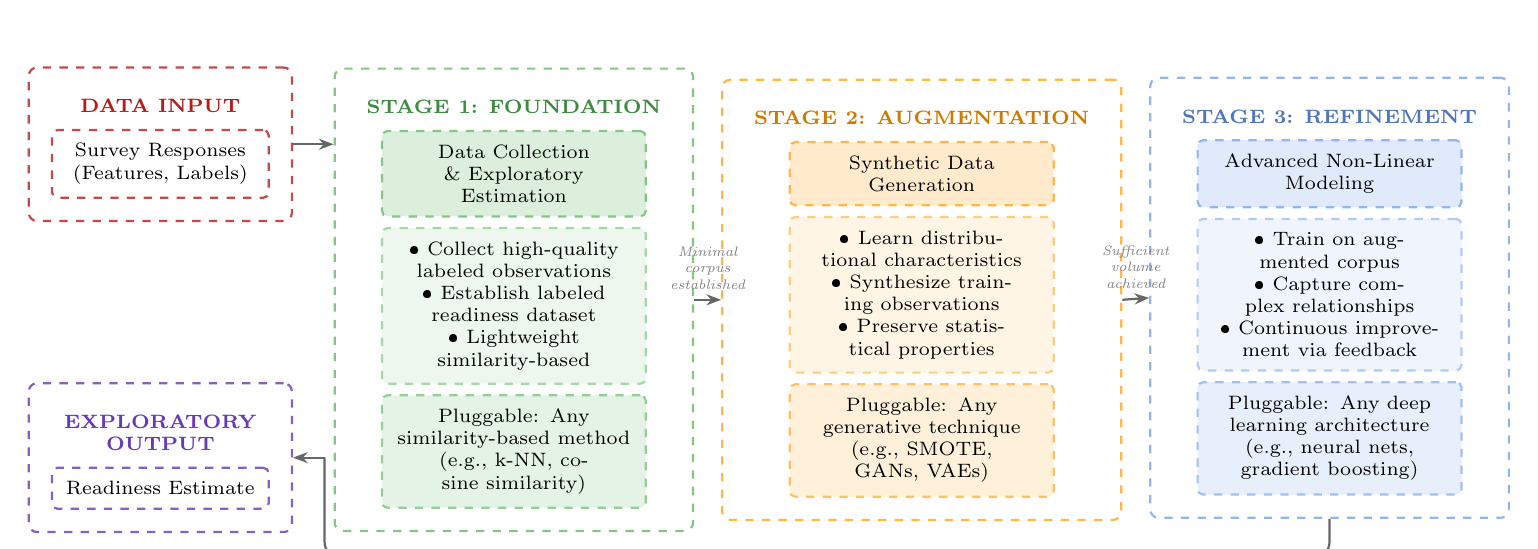
\begin{tikzpicture}[
    node distance=0.3cm,
    inner/.style={rectangle, dashed, thick, rounded corners=2pt, align=center, inner sep=5pt, font=\scriptsize},
    outer/.style={rectangle, dashed, thick, rounded corners=3pt, inner sep=8pt},
    header/.style={inner, fill=#1!20, draw=#1!70},
    content/.style={inner, fill=#1!10, draw=#1!50},
    plug/.style={inner, fill=#1!15, draw=#1!60},
    arrow/.style={-{Stealth[scale=0.8]}, black!60, thick},
    lbl/.style={font=\tiny\itshape, text=black!50, align=center}
]

\node[header=stage1, text width=3cm, minimum height=0.8cm] (s1-head) {Data Collection \& Exploratory\\Estimation};
\node[content=stage1, below=0.12cm of s1-head, text width=3cm, minimum height=1.4cm] (s1-content) {
    \textbullet\ Collect high-quality labeled observations\\
    \textbullet\ Establish labeled readiness dataset\\
    \textbullet\ Lightweight similarity-based
};
\node[plug=stage1, below=0.12cm of s1-content, text width=3cm, minimum height=0.9cm] (s1-plug) {Pluggable: Any\\similarity-based method\\(e.g., k-NN, cosine similarity)};
\node[above=0.08cm of s1-head, font=\scriptsize\bfseries, text=stage1!80!black] (s1-title) {STAGE 1: FOUNDATION};
\node[outer, draw=stage1!70, fit=(s1-title)(s1-head)(s1-content)(s1-plug)] (stage1-box) {};

\node[header=stage2, right=1.8cm of s1-head, text width=3cm, minimum height=0.8cm] (s2-head) {Synthetic Data\\Generation};
\node[content=stage2, below=0.12cm of s2-head, text width=3cm, minimum height=1.4cm] (s2-content) {
    \textbullet\ Learn distributional characteristics\\
    \textbullet\ Synthesize training observations\\
    \textbullet\ Preserve statistical properties
};
\node[plug=stage2, below=0.12cm of s2-content, text width=3cm, minimum height=0.9cm] (s2-plug) {Pluggable: Any\\generative technique\\(e.g., SMOTE, GANs, VAEs)};
\node[above=0.08cm of s2-head, font=\scriptsize\bfseries, text=stage2!80!black] (s2-title) {STAGE 2: AUGMENTATION};
\node[outer, draw=stage2!70, fit=(s2-title)(s2-head)(s2-content)(s2-plug)] (stage2-box) {};

\node[header=stage3, right=1.8cm of s2-head, text width=3cm, minimum height=0.8cm] (s3-head) {Advanced Non-Linear\\Modeling};
\node[content=stage3, below=0.12cm of s3-head, text width=3cm, minimum height=1.4cm] (s3-content) {
    \textbullet\ Train on augmented corpus\\
    \textbullet\ Capture complex relationships\\
    \textbullet\ Continuous improvement via feedback
};
\node[plug=stage3, below=0.12cm of s3-content, text width=3cm, minimum height=0.9cm] (s3-plug) {Pluggable: Any deep\\learning architecture\\(e.g., neural nets, gradient boosting)};
\node[above=0.08cm of s3-head, font=\scriptsize\bfseries, text=stage3!80!black] (s3-title) {STAGE 3: REFINEMENT};
\node[outer, draw=stage3!70, fit=(s3-title)(s3-head)(s3-content)(s3-plug)] (stage3-box) {};



\node[font=\scriptsize\bfseries, text=inputred, anchor=north] (input-title) at ([xshift=-2.2cm, yshift=-8pt]stage1-box.north west) {DATA INPUT};
\node[inner, fill=white, draw=inputred!80, text width=2.4cm, below=0.08cm of input-title] (input-inner) {Survey Responses\\(Features, Labels)};
\node[outer, draw=inputred!80, fit=(input-title)(input-inner)] (input-box) {};

\node[inner, fill=white, draw=outputviolet!80, text width=2.4cm, anchor=south] (output-inner) at ([xshift=-2.2cm, yshift=8pt]stage1-box.south west) {Readiness Estimate};
\node[above=0.08cm of output-inner, font=\scriptsize\bfseries, text=outputviolet, align=center] (output-title) {EXPLORATORY\\OUTPUT};
\node[outer, draw=outputviolet!80, fit=(output-title)(output-inner)] (output-box) {};

\draw[arrow] (input-box.east) -- (stage1-box.west |- input-box.east);
\draw[arrow] (stage1-box.east) -- node[lbl, above] {Minimal\\corpus\\established} (stage2-box.west);
\draw[arrow] (stage2-box.east) -- node[lbl, above] {Sufficient\\volume\\achieved} (stage3-box.west);

\coordinate (turn1) at ([yshift=-0.5cm]stage3-box.south);
\coordinate (turn2) at (turn1 -| output-box.east);
\coordinate (turn3) at ([xshift=0.4cm]output-box.east);
\draw[black!60, thick, rounded corners=6pt] (stage3-box.south) -- (turn1) -- (turn1 -| turn3) -- (turn3);
\draw[arrow] (turn3) -- (output-box.east);

\end{tikzpicture}
}\end{figure}

\begin{quote}\footnotesize
\textit{Diagram text changes:} \DIFadd{The} \DIFadd{Three-Stage} \DIFadd{Progressive} \DIFadd{Pipeline.} \DIFadd{Each} \DIFadd{stage} \DIFadd{represents} \DIFadd{a} \DIFadd{pluggable} \DIFadd{component} \DIFadd{that} \DIFadd{can} \DIFadd{be} \DIFadd{substituted} \DIFadd{with} \DIFadd{alternative} \DIFadd{algorithms.} \DIFadd{The} \DIFadd{framework} \DIFadd{progresses} \DIFadd{from} \DIFadd{data} \DIFadd{acquisition} \DIFadd{through} \DIFadd{augmentation} \DIFadd{to} \DIFadd{refined} \DIFadd{prediction,} \DIFadd{with} \DIFadd{feedback} \DIFadd{loops} \DIFadd{enabling} \DIFadd{continuous} \DIFadd{improvement.}; Data Collection \& \DIFdel{Initial} \DIFadd{Exploratory} \DIFdel{Prediction;} \DIFadd{Estimation;} Pluggable: Any similarity-based method (e.g., k-NN, cosine similarity); STAGE 1: FOUNDATION; Synthetic Data Generation; Pluggable: Any generative technique (e.g., SMOTE, GANs, VAEs); STAGE 2: AUGMENTATION; Advanced Non-Linear Modeling; Pluggable: Any deep learning architecture (e.g., neural nets, gradient boosting); STAGE 3: REFINEMENT; DATA INPUT; Survey Responses (Features, Labels); Readiness \DIFdel{Score;} \DIFadd{Estimate;} \DIFdel{PREDICTION} \DIFadd{EXPLORATORY} OUTPUT
\end{quote}

\subsection{Configuration Flexibility}\label{subsec:config}

The modular pipeline design described above is \DIFdel{implemented} \DIFadd{supported} \DIFdel{through} \DIFadd{by} a configuration system that allows researchers to adapt the framework without modifying the core infrastructure. Four categories of settings \DIFdel{support} \DIFadd{provide} this flexibility:

\textbf{Survey Linkage:} The dual-survey architecture uses explicit linkage settings. A single Target Survey (\DIFdel{outcome} \DIFadd{readiness} \DIFadd{measure} $Y$) may be linked to multiple Factor Surveys (predictor sets $X_1, X_2, X_3$), which allows researchers to examine which predictor combinations perform \DIFdel{best.} \DIFadd{best} \DIFadd{once} \DIFadd{suitable} \DIFadd{longitudinal} \DIFadd{outcomes} \DIFadd{exist.} Figure~\ref{fig:linkage} shows how linked surveys flow into the model during training and prediction. This arrangement provides several practical advantages:

\begin{enumerate}
    \item \textbf{Comparative predictor analysis:} researchers can deploy alternative Factor Surveys to the same cohort and compare \DIFdel{predictive} \DIFadd{their} validity \DIFdel{across} \DIFadd{once} \DIFdel{predictor} \DIFadd{suitable} \DIFdel{sets;} \DIFadd{outcomes} \DIFadd{exist;}
    \item \textbf{Longitudinal adaptability:} as research identifies new predictors of transfer success, new Factor Surveys can be added without disrupting existing data collection or invalidating earlier comparisons;
    \item \textbf{Cohort customization:} different academic programs can deploy program-specific Factor Surveys while maintaining a common outcome measure through shared Target Surveys.
\end{enumerate}

\begin{figure}[htbp]
\centering
\caption{Dual-Survey Architecture with survey linkage. Gray arrows show the Target Survey readiness measure and Factor Survey predictors entering model training, while green arrows show Factor Survey predictors passing through inference. Dashed lines show linkage relationships between Target and Factor Surveys.}
\label{fig:linkage}
\resizebox{0.67\textwidth}{!}{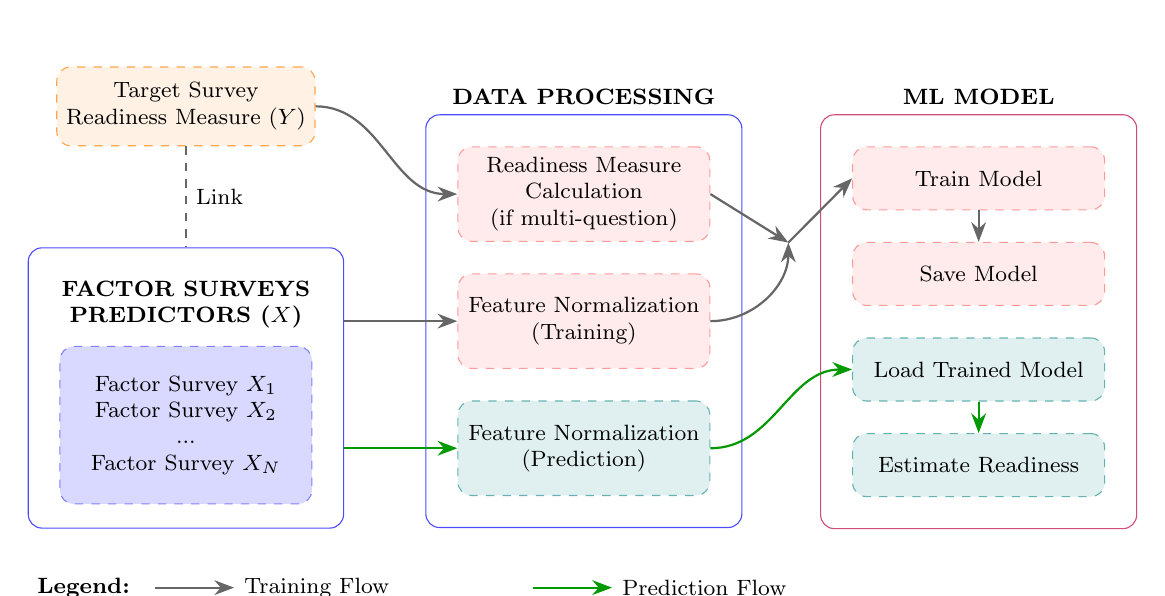
\begin{tikzpicture}[
  box/.style={draw,dashed,rounded corners=5pt,align=center,font=\footnotesize},
  container/.style={draw,rounded corners=5pt,inner sep=4mm},
    trainbox/.style={box,draw=red!40,fill=red!8},
  trainarr/.style={black!60,thick,-{Stealth[length=2.5mm]}},
    predbox/.style={box,draw=teal!60,fill=teal!12},
  predarr/.style={green!60!black,thick,-{Stealth[length=2.5mm]}}
]
\node[box,draw=orange!70,fill=orange!10,minimum width=32mm,minimum height=10mm] (target) {Target Survey\\Readiness Measure ($Y$)};

\node[trainbox,minimum width=32mm,minimum height=12mm,right=18mm of target.south east,anchor=north west] (weighted) {Readiness Measure\\Calculation\\(if multi-question)};
\node[trainbox,minimum width=32mm,minimum height=12mm,below=4mm of weighted] (normtrain) {Feature Normalization\\(Training)};
\node[predbox,minimum width=32mm,minimum height=12mm,below=4mm of normtrain] (normpred) {Feature Normalization\\(Prediction)};
\node[container,draw=blue!70,fit=(weighted)(normtrain)(normpred),label={[font=\footnotesize\bfseries]above:DATA PROCESSING}] (dbox) {};

\node[box,draw=blue!50,fill=blue!15,minimum width=32mm,minimum height=20mm,anchor=south] at ([yshift=3mm]target.south|-dbox.south) (factors) {Factor Survey $X_1$\\Factor Survey $X_2$\\...\\Factor Survey $X_N$};
\node[font=\footnotesize\bfseries,align=center,above=1mm of factors] (flabel) {FACTOR SURVEYS\\PREDICTORS ($X$)};
\node[container,draw=blue!70,inner sep=3mm,fit=(factors)(flabel)] (fbox) {};

\draw[black!60,dashed,thick] (target.south) -- node[right,font=\footnotesize,black]{Link} (fbox.north);

\node[trainbox,minimum width=32mm,minimum height=8mm,right=18mm of weighted.north east,anchor=north west] (train) {Train Model};
\node[trainbox,minimum width=32mm,minimum height=8mm,below=4mm of train] (save) {Save Model};
\node[predbox,minimum width=32mm,minimum height=8mm,below=4mm of save] (load) {Load Trained Model};
\node[predbox,minimum width=32mm,minimum height=8mm,below=4mm of load] (predict) {Estimate Readiness};
\node[container,draw=purple!70,fit=(train)(save)(load)(predict),label={[font=\footnotesize\bfseries]above:ML MODEL}] (mbox) {};

\draw[trainarr] (target.east) to[out=0,in=180] (weighted.west);
\draw[trainarr] (fbox.east |- normtrain.west) -- (normtrain.west);
\coordinate (trainmerge) at ($(normtrain.east)!0.55!(train.west)$ |- train.west);
\draw[trainarr] (weighted.east) -- (trainmerge);
\draw[trainarr] (normtrain.east) to[out=0,in=-90] (trainmerge);
\draw[trainarr] (trainmerge) -- (train.west);
\draw[trainarr] (train.south) -- (save.north);

\draw[predarr] (fbox.east |- normpred.west) -- (normpred.west);
\draw[predarr] (normpred.east) to[out=0,in=180] (load.west);
\draw[predarr] (load.south) -- (predict.north);

\node[below=5mm of fbox.south west,anchor=north west,font=\footnotesize\bfseries] (legendlabel) {Legend:};
\draw[trainarr] ([xshift=2mm]legendlabel.east) -- ++(10mm,0) node[right,font=\footnotesize,black] {Training Flow};
\node[right=50mm of legendlabel.east,anchor=west] (predlegendstart) {};
\draw[predarr] (predlegendstart.west) -- ++(10mm,0) node[right,font=\footnotesize,black] {Prediction Flow};
\end{tikzpicture}
}\end{figure}

\begin{quote}\footnotesize
\textit{Diagram text changes:} \DIFadd{Dual-Survey} \DIFadd{Architecture} \DIFadd{with} \DIFadd{survey} \DIFadd{linkage.} \DIFadd{Gray} \DIFadd{arrows} \DIFadd{show} \DIFadd{the} Target Survey \DIFadd{readiness} \DIFadd{measure} \DIFadd{and} \DIFadd{Factor} \DIFadd{Survey} \DIFadd{predictors} \DIFadd{entering} \DIFadd{model} \DIFadd{training,} \DIFadd{while} \DIFadd{green} \DIFadd{arrows} \DIFadd{show} \DIFadd{Factor} \DIFadd{Survey} \DIFadd{predictors} \DIFadd{passing} \DIFadd{through} \DIFadd{inference.} \DIFadd{Dashed} \DIFadd{lines} \DIFadd{show} \DIFadd{linkage} \DIFadd{relationships} \DIFadd{between} \DIFadd{Target} \DIFadd{and} \DIFadd{Factor} \DIFadd{Surveys.}; \DIFadd{Target} \DIFadd{Survey} \DIFadd{Readiness} \DIFadd{Measure} (\DIFdel{Label} $\DIFadd{Y}$); \DIFdel{Weighted} \DIFadd{Readiness} \DIFadd{Measure} Calculation (if multi-question); Feature Normalization (Training); Feature Normalization (Prediction); Factor Survey $X_1$ Factor Survey $X_2$ ... Factor Survey $X_N$; FACTOR SURVEYS \DIFadd{PREDICTORS} (\DIFdel{Features} $\DIFadd{X}$); Train Model; Save Model; Load Trained Model; \DIFdel{Predict} \DIFadd{Estimate} Readiness; Legend:
\end{quote}

The remaining three categories address the progressive learning pipeline:

\textbf{Phase Transition Thresholds.} Administrators specify how many observations are required before the system moves from one pipeline stage to the next. Default thresholds reflect statistical considerations for each algorithm family, but institutions can adjust them based on enrollment patterns and the desired balance between prediction availability and model reliability.

\textbf{Algorithm Selection:} Each pipeline stage \DIFdel{accepts} \DIFadd{is} \DIFadd{designed} \DIFadd{to} \DIFadd{accept} any algorithm that matches the expected interface. The \textbf{foundation stage} requires a predictor that works with minimal training data. The \textbf{augmentation stage} requires a generative model that can synthesize observations while preserving the main properties of the data. The \textbf{refinement stage} accepts supervised learning architectures that can capture non-linear relationships. This modularity allows researchers to compare alternatives on their own student populations rather than rely on fixed defaults.

\textbf{Hyperparameter Tuning:} Within each algorithm, configurable parameters \DIFadd{can} support fine-tuning for institutional context. Distance metrics, neighbor counts, generation multipliers, network architectures, and training schedules are all exposed as settings. The system logs each configuration together with model performance metrics to support systematic comparison.

This configuration structure \DIFdel{allows} \DIFadd{is} \DIFadd{intended} \DIFadd{to} \DIFadd{allow} institutions to adopt newer methods, including improved few-shot learning techniques, stronger data augmentation strategies, or newer model architectures, by updating settings rather than reengineering the full system.

\section{Evaluation}\label{sec:evaluation}

To assess the usability and perceived value of ACOSUS, we conducted a pilot study with transfer students at a public urban university. This section describes the study design, evaluation instruments, quantitative results, and qualitative findings.

\subsection{Study Design}\label{subsec:studydesign}

Ten transfer students ($N=10$) from public universities in the United States participated in the study. Participants were recruited by email and enrolled after providing informed consent. All were active transfer students in computing-related majors. The evaluation took place during the foundation phase of the progressive learning pipeline, when the system was still collecting labeled observations for the initial training corpus. At that stage, no predictive model had yet been trained, so the system's main function was structured data collection rather than prediction. Participants completed the Factor and Target Survey instruments, then completed a feedback survey through Qualtrics. The study protocol received Institutional Review Board (IRB) approval before data collection began. \DIFadd{The} \DIFadd{pilot} \DIFadd{evaluated} \DIFadd{the} \DIFadd{student-facing} \DIFadd{interface} \DIFadd{and} \DIFadd{survey} \DIFadd{workflow,} \DIFadd{rather} \DIFadd{than} \DIFadd{predictive} \DIFadd{validity,} \DIFadd{advisor-dashboard} \DIFadd{usability,} \DIFadd{longitudinal} \DIFadd{outcomes,} \DIFadd{fairness,} \DIFadd{or} \DIFadd{institutional} \DIFadd{deployment.}

\subsection{Evaluation Instruments}\label{subsec:instruments}

The feedback survey was based on the Technology Acceptance Model (TAM) framework \parencite{davis1989} and was used to assess participants' perceptions of the data collection experience. It included 5-point Likert-scale items measuring Perceived Usefulness, Perceived Ease of Use, and Behavioral Intention, along with open-ended questions about interface difficulties, helpful features, missing capabilities, and redesign suggestions. Table~\ref{tab:constructs} presents the constructs and example items.

\begin{table}[htbp]
\centering
\caption{Feedback survey constructs and \DIFdel{items.} \DIFadd{items}}
\label{tab:constructs}
 \begin{tabularx}{\textwidth}{@{}>{\hsize=.65\hsize\linewidth=\hsize}Y>{\hsize=1.35\hsize\linewidth=\hsize}Y@{}}
\toprule
\textbf{Construct} & \textbf{Example Item} \\
\midrule
Perceived Usefulness (PU) & ``Using this AI counseling system enables me to accomplish tasks more quickly than other advising methods.'' \\
Perceived Ease of Use (PEOU) & ``Learning to operate this AI counseling system was easy for me.'' \\
Behavioral Intention & ``How likely are you to continue using this system for academic planning?'' \\
\bottomrule
 \end{tabularx}
\end{table}

Open-ended questions captured qualitative feedback on interface difficulties, helpful features, missing capabilities, and redesign suggestions.

\subsection{Quantitative Results}\label{subsec:quantresults}

\subsubsection{TAM Construct Scores}

The TAM-based measures showed favorable responses on perceived ease of use and perceived usefulness across the participant group (Table~\ref{tab:results}). Because this evaluation was conducted during the foundation phase, before any predictive output had been generated for participants, the scores reflect participants' experience of the data-collection workflow and interface rather than the system's predictive utility. Lower ratings on usefulness should therefore be read as a reflection of the system's current functionality at the foundation phase rather than as evidence against the underlying design.

\begin{table}[htbp]
\centering
\caption{Summary statistics for evaluation metrics (5-point Likert scale)}
\label{tab:results}
 \begin{tabularx}{\textwidth}{@{}Ycccc@{}}
\toprule
\textbf{Metric} & \textbf{Mean} & \textbf{SD} & \textbf{Min} & \textbf{Max} \\
\midrule
Perceived Usefulness (PU) & 3.37 & 1.29 & 1 & 5 \\
Perceived Ease of Use (PEOU) & 4.13 & 1.05 & 1 & 5 \\
Likelihood to Continue & 3.12 & 1.89 & 1 & 5 \\
Likelihood to Recommend & 3.00 & 1.77 & 1 & 5 \\
 \midrule
 \multicolumn{5}{@{}p{\textwidth}@{}}{\footnotesize\textit{Note.} Behavioral-intention items have $N=8$; two participants did not provide a usable rating.} \\
\bottomrule
 \end{tabularx}
\end{table}

\begin{figure}[htbp]
\centering
\caption{TAM construct scores ($N=10$). Perceived Ease of Use was the highest-rated TAM construct ($M=4.13$), while Perceived Usefulness was lower and more dispersed ($M=3.37$).}
\label{fig:tam}

\includegraphics[width=0.72\textwidth]{infographics/fig1_tam_metrics.png}
\end{figure}

As Figure~\ref{fig:tam} shows, Perceived Ease of Use received the highest mean among the TAM constructs ($M=4.13$, $SD=1.05$), indicating positive agreement that the system is easy to learn and use, with relatively consistent responses across participants. Perceived Usefulness was lower and more dispersed ($M=3.37$, $SD=1.29$), suggesting that participants saw the system as easy to operate but were less uniformly convinced of its usefulness for their own advising needs.

\subsubsection{Behavioral Intention}

\begin{figure}[htbp]
\centering
\caption{Behavioral intention ($N=8$). Likelihood to Continue ($M=3.12$) was slightly higher than Likelihood to Recommend ($M=3.00$); both showed substantial variance across respondents ($SD\approx1.8$).}
\label{fig:behavioral}

\includegraphics[width=0.78\textwidth]{infographics/fig4_behavioral_intention.png}
\end{figure}

Behavioral intention was the weakest dimension in the evaluation (Figure~\ref{fig:behavioral}). Likelihood to Continue using the system was moderate on average ($M=3.12$, $SD=1.89$), and Likelihood to Recommend was slightly lower and similarly dispersed ($M=3.00$, $SD=1.77$). Two participants \DIFdel{did} \DIFdel{not} \DIFdel{provide} \DIFdel{a} \DIFadd{lacked} usable \DIFdel{rating} \DIFadd{ratings} for these \DIFdel{items} \DIFadd{items,} \DIFdel{and} \DIFdel{are} \DIFdel{excluded} \DIFdel{from} \DIFadd{so} the behavioral-intention means  \DIFadd{use} $N=8$. \DIFdel{Both} \DIFdel{distributions} \DIFdel{are} \DIFdel{bimodal:} \DIFdel{several} \DIFdel{respondents} \DIFdel{scored} \DIFdel{5}\DIFdel{5} \DIFdel{while} \DIFdel{others} \DIFdel{scored} \DIFdel{1}\DIFdel{--}\DIFdel{2,} \DIFdel{with} \DIFdel{few} \DIFdel{intermediate} \DIFdel{ratings.} \DIFdel{This} \DIFdel{pattern} \DIFdel{suggests} \DIFdel{that} \DIFdel{the} \DIFdel{system} \DIFdel{appeals} \DIFdel{strongly} \DIFdel{to} \DIFdel{a} \DIFdel{subset} \DIFdel{of} \DIFdel{transfer} \DIFdel{students} \DIFdel{but} \DIFdel{not} \DIFdel{to} \DIFdel{others,} \DIFdel{rather} \DIFdel{than} \DIFdel{producing} \DIFdel{uniform} \DIFdel{mild} \DIFdel{enthusiasm.} \DIFdel{We} \DIFdel{read} \DIFdel{this} \DIFdel{cautiously:} \DIFdel{with} \DIFdel{only} \DIFdel{a} \DIFdel{small} \DIFdel{number} \DIFdel{of} \DIFdel{respondents} \DIFdel{at} \DIFdel{the} \DIFdel{foundation} \DIFdel{phase,} \DIFdel{when} \DIFdel{no} \DIFdel{predictions} \DIFdel{had} \DIFdel{yet} \DIFdel{been} \DIFdel{generated,} \DIFdel{low} \DIFdel{recommendation} \DIFdel{scores} \DIFdel{may} \DIFdel{reflect} \DIFdel{limited} \DIFdel{current} \DIFdel{utility} \DIFdel{rather} \DIFdel{than} \DIFdel{rejection} \DIFdel{of} \DIFdel{the} \DIFdel{design.}

\DIFadd{Both} \DIFadd{distributions} \DIFadd{are} \DIFadd{bimodal:} \DIFadd{several} \DIFadd{respondents} \DIFadd{scored} \DIFadd{5}/\DIFadd{5} \DIFadd{while} \DIFadd{others} \DIFadd{scored} \DIFadd{1}\DIFadd{--}\DIFadd{2,} \DIFadd{with} \DIFadd{few} \DIFadd{intermediate} \DIFadd{ratings.} \DIFadd{This} \DIFadd{pattern} \DIFadd{suggests} \DIFadd{that} \DIFadd{the} \DIFadd{system} \DIFadd{appeals} \DIFadd{strongly} \DIFadd{to} \DIFadd{a} \DIFadd{subset} \DIFadd{of} \DIFadd{transfer} \DIFadd{students} \DIFadd{but} \DIFadd{not} \DIFadd{to} \DIFadd{others,} \DIFadd{rather} \DIFadd{than} \DIFadd{producing} \DIFadd{uniform} \DIFadd{mild} \DIFadd{enthusiasm.} \DIFadd{We} \DIFadd{read} \DIFadd{this} \DIFadd{cautiously:} \DIFadd{with} \DIFadd{only} \DIFadd{a} \DIFadd{small} \DIFadd{number} \DIFadd{of} \DIFadd{respondents} \DIFadd{at} \DIFadd{the} \DIFadd{foundation} \DIFadd{phase,} \DIFadd{when} \DIFadd{no} \DIFadd{predictions} \DIFadd{had} \DIFadd{yet} \DIFadd{been} \DIFadd{generated,} \DIFadd{low} \DIFadd{recommendation} \DIFadd{scores} \DIFadd{may} \DIFadd{reflect} \DIFadd{limited} \DIFadd{current} \DIFadd{utility} \DIFadd{rather} \DIFadd{than} \DIFadd{rejection} \DIFadd{of} \DIFadd{the} \DIFadd{design.}

\DIFadd{For} \DIFadd{each} \DIFadd{respondent,} \DIFadd{we} \DIFadd{averaged} \DIFadd{the} \DIFadd{available} \DIFadd{behavioral-intention} \DIFadd{items.} \DIFadd{We} \DIFadd{classified} \DIFadd{means} \DIFadd{of} \DIFadd{4} \DIFadd{or} \DIFadd{higher} \DIFadd{as} \DIFadd{high} \DIFadd{intention,} \DIFadd{2} \DIFadd{or} \DIFadd{lower} \DIFadd{as} \DIFadd{low} \DIFadd{intention,} \DIFadd{and} \DIFadd{values} \DIFadd{between} \DIFadd{those} \DIFadd{thresholds} \DIFadd{as} \DIFadd{intermediate.} \DIFadd{One} \DIFadd{respondent} \DIFadd{was} \DIFadd{missing} \DIFadd{both} \DIFadd{items.} \DIFadd{Table}~\DIFaddcite{\ref{tab:subgroups} }\DIFadd{reports} \DIFadd{aggregate} \DIFadd{means} \DIFadd{only.}

\begin{table}[htbp]
\caption{Exploratory behavioral-intention subgroup means}
\label{tab:subgroups}
\centering
\begin{tabular*}{\textwidth}{@{\extracolsep{\fill}}lrrrrrrr@{}}
\toprule
\textbf{Group} & \textbf{$N$} & \textbf{PU} & \textbf{PEOU} & \textbf{Accuracy} & \textbf{Alignment} & \textbf{Relevance} & \textbf{Actionability} \\
\midrule
High intention & 3 & 4.83 & 5.00 & 4.67 & 4.67 & 4.67 & 5.00 \\
Low intention & 4 & 2.71 & 3.62 & 2.25 & 2.00 & 2.25 & 2.50 \\
Intermediate & 2 & 2.92 & 3.75 & 4.50 & 3.00 & 2.50 & 3.00 \\
Missing both items & 1 & 2.50 & 4.33 & 4.00 & -- & 3.00 & 2.00 \\
\bottomrule
\end{tabular*}
\end{table}

\DIFadd{The} \DIFadd{subgroup} \DIFadd{averages} \DIFadd{were} \DIFadd{consistent} \DIFadd{with} \DIFadd{the} \DIFadd{spread} \DIFadd{in} \DIFadd{behavioral} \DIFadd{intention.} \DIFadd{High-intention} \DIFadd{respondents} \DIFadd{rated} \DIFadd{both} \DIFadd{usability} \DIFadd{and} \DIFadd{perceived} \DIFadd{advising} \DIFadd{value} \DIFadd{highly.} \DIFadd{Low-intention} \DIFadd{respondents} \DIFadd{still} \DIFadd{rated} \DIFadd{ease} \DIFadd{of} \DIFadd{use} \DIFadd{above} \DIFadd{the} \DIFadd{scale} \DIFadd{midpoint} \DIFadd{but} \DIFadd{reported} \DIFadd{lower} \DIFadd{usefulness,} \DIFadd{accuracy,} \DIFadd{alignment,} \DIFadd{relevance,} \DIFadd{and} \DIFadd{actionability.} \DIFadd{Their} \DIFadd{open-ended} \DIFadd{comments} \DIFadd{emphasized} \DIFadd{missing} \DIFadd{course} \DIFadd{or} \DIFadd{prerequisite} \DIFadd{analysis,} \DIFadd{deeper} \DIFadd{career} \DIFadd{exploration,} \DIFadd{or} \DIFadd{a} \DIFadd{preference} \DIFadd{for} \DIFadd{human} \DIFadd{advising.} \DIFadd{Given} \DIFadd{the} \DIFadd{very} \DIFadd{small} \DIFadd{groups,} \DIFadd{these} \DIFadd{comparisons} \DIFadd{are} \DIFadd{descriptive} \DIFadd{only.} \DIFadd{No} \DIFadd{significance} \DIFadd{tests} \DIFadd{were} \DIFadd{performed,} \DIFadd{and} \DIFadd{the} \DIFadd{pattern} \DIFadd{cannot} \DIFadd{support} \DIFadd{population-level} \DIFadd{conclusions.}

\subsection{Qualitative Findings}\label{subsec:qualfindings}

Open-ended responses yielded five main themes, whose frequencies are shown in Figure~\ref{fig:themes} and whose representative quotes appear in Table~\ref{tab:themes}.

\begin{figure}[htbp]
\centering
\caption{Qualitative theme distribution ($N$=10). Feature Requests was the most frequent theme (7 mentions), followed by UI/Navigation Positive (6), No Issues Reported (5), Assessment \& Exploration Value (4), and a single expression of Preference for Human Advising (1).}
\label{fig:themes}

\includegraphics[width=0.72\textwidth]{infographics/fig6_qualitative_themes.png}
\end{figure}

\begin{table}[htbp]
\centering
\caption{Qualitative themes and representative responses ($N=10$).}
\label{tab:themes}
 \begin{tabularx}{\textwidth}{@{}>{\hsize=.70\hsize\linewidth=\hsize}Yc>{\hsize=1.30\hsize\linewidth=\hsize}Y@{}}
\toprule
\textbf{Theme} & \textbf{Count} & \textbf{Representative Quote} \\
\midrule
Feature Requests & 7 & ``Make it tailored more towards individual users and their specific situation''; ``Better analysis of prerequisites to allow for registration'' \\
UI/Navigation Positive & 6 & ``The UI navigation is very user friendly''; ``All the interface of the website was very intuitive to interact with'' \\
No Issues Reported & 5 & ``No feature was missing, my experience was great''; ``None, everything was clear'' \\
Assessment \& Exploration Value & 4 & ``The assessment is fun and helpful to me''; ``Career exploration'' \\
Preference for Human Advising & 1 & ``I have never had a problem with a human advisor. Please don't replace a human being with AI'' \\
\bottomrule
 \end{tabularx}
\end{table}

\textbf{Feature Requests} was the most frequent theme. Rather than indicating dissatisfaction, the pattern suggests that participants engaged closely enough with the system to want it to do more. Several asked for tighter personalization, with one participant writing that they would ``make it tailored more towards individual users and their specific situation,'' while others requested deeper academic functionality, such as ``better analysis of prerequisites to allow for registration'' and ``more answer choices besides the ones provided.'' \textbf{UI/Navigation Positive} was the next most common theme; participants consistently described the interface as easy to navigate, with one writing that ``the UI navigation is very user friendly'' and another that ``all the interface of the website was very intuitive to interact with,'' which is consistent with PEOU being the highest-rated TAM construct ($M=4.13$). \textbf{No Issues Reported} formed a third cluster: when asked about missing features or interface difficulties, several participants responded with comments such as ``no feature was missing, my experience was great'' and ``none, everything was clear.'' Finally, \textbf{Assessment \& Exploration Value} captured comments in which participants recognized the system's worth for self-assessment and for exploring their options, even at the foundation phase when no predictions were yet available; participants described it as a tool for ``career exploration'' and noted that ``the assessment is fun and helpful to me.'' A fifth theme emerged from a single, more skeptical participant, who wrote that they ``have never had a problem with a human advisor'' and \DIFdel{asking} \DIFadd{asked} that the system ``not replace a human being with AI.'' Although isolated, this comment reflects a \textbf{Preference for Human Advising} and echoes the advisors' own view that the system should complement rather than substitute for human advising.

Alongside the student pilot, the project also received informal feedback from academic advisors. Advisors agreed that the system addresses a real need and viewed it as a promising direction, while noting that its full value depends on the prediction capability that the foundation phase has not yet produced. They also indicated that the system could help students arrive better prepared for advising meetings, and that consolidating its captured information into a single advising hub would further strengthen its value to advising workflows. \DIFadd{These} \DIFadd{comments} \DIFadd{motivate} \DIFadd{formal} \DIFadd{advisor} \DIFadd{testing,} \DIFadd{but} \DIFadd{they} \DIFadd{were} \DIFadd{not} \DIFadd{collected} \DIFadd{through} \DIFadd{a} \DIFadd{defined} \DIFadd{advisor} \DIFadd{sample} \DIFadd{or} \DIFadd{usability} \DIFadd{protocol} \DIFadd{and} \DIFadd{are} \DIFadd{not} \DIFadd{treated} \DIFadd{as} \DIFadd{evaluation} \DIFadd{evidence.}

\section{Conclusion and Future Work}\label{sec:conclusion}

This paper presented ACOSUS, an AI-driven counseling system designed for transfer students in computing majors. The system addresses two problems that often limit transfer advising: fragmented information and limited institutional data for prediction.

Our primary contributions are: (1) a dual-survey architecture that separates \DIFdel{outcome} \DIFadd{readiness} measurement from predictor \DIFadd{collection;} (\DIFadd{2}) \DIFadd{structured} \DIFadd{transfer-specific} \DIFadd{data} collection \DIFdel{while} \DIFadd{and} \DIFdel{providing} \DIFdel{advisors} \DIFdel{with} \DIFdel{structured} \DIFadd{organized} student profiles through a unified \DIFadd{advisor} dashboard; (\DIFdel{2} \DIFadd{3}) a modular prediction architecture with configuration support for survey linkage, phase transitions, and hyperparameters, allowing institutions to adapt the system to their own settings; and (\DIFdel{3} \DIFadd{4}) a pilot evaluation with transfer students ($N=10$) showing that the system is perceived as moderately easy to use and useful, with Perceived Ease of Use ($M=4.13$) the strongest of the TAM constructs, alongside notable variance in behavioral intention. \DIFadd{The} \DIFadd{dashboard} \DIFadd{is} \DIFadd{implemented,} \DIFadd{but} \DIFadd{it} \DIFadd{was} \DIFadd{not} \DIFadd{formally} \DIFadd{evaluated} \DIFadd{in} \DIFadd{the} \DIFadd{pilot.}

The system is currently operational and collecting observations during the foundation phase, but its predictive components still need to be evaluated as the dataset grows. The pilot's small sample size ($N=10$), small number of participating institutions, voluntary enrollment, and cross-sectional design limit generalizability, and longitudinal outcome tracking was beyond the scope of the present study. \DIFadd{Dashboard} \DIFadd{usability,} \DIFadd{fairness,} \DIFadd{and} \DIFadd{multi-institutional} \DIFadd{validation} \DIFadd{also} \DIFadd{remain} \DIFadd{to} \DIFadd{be} \DIFadd{evaluated.}

Future work includes: (1) evaluating the full progressive pipeline once sufficient observations have been collected, including accuracy, calibration, and fairness; (2) deploying the system across multiple institutions to test generalizability; (3) incorporating advisor feedback into the prediction process and evaluating dashboard use in practice; and (4) exploring LLM-based narrative explanations and intervention recommendations.

Taken together, these design choices suggest a practical approach to deploying intelligent advising systems in educational settings where data are limited at the outset. \DIFadd{The} \DIFadd{present} \DIFadd{pilot} \DIFadd{supports} \DIFadd{the} \DIFadd{design} \DIFadd{feasibility} \DIFadd{of} \DIFadd{the} \DIFadd{student-facing} \DIFadd{interface} \DIFadd{and} \DIFadd{survey} \DIFadd{workflow,} \DIFadd{not} \DIFadd{predictive} \DIFadd{validity} \DIFadd{or} \DIFadd{improvement} \DIFadd{in} \DIFadd{longitudinal} \DIFadd{student} \DIFadd{success.}

\section{Acknowledgments}

\small

This material is based upon work supported by the National Science Foundation under Grant No. CNS-2219623.

\begin{sloppypar}
\clearpage

\section{Bibliography Changes}

This summary compares works cited in the submitted version with works cited in the final draft.

\subsection{Added Citations}

\DIFaddedreference{assistResource2026}

\DIFaddedreference{collegeSourceTES2026}

\DIFaddedreference{mattei2014advising}

\DIFaddedreference{mi2025smartcourse}

\DIFaddedreference{navigate3602026}

\DIFaddedreference{nguyen2024optimal}

\DIFaddedreference{transferologySupport2026}

\subsection{Removed Citations}

\DIFremovedreference{bandura1997}

\DIFremovedreference{tinto1993}

\clearpage

\printbibliography[title={REFERENCES}]
\end{sloppypar}

\end{document}
